
\documentclass{article}
\usepackage{xcolor}
\usepackage{pgf-pie}
\usepackage{ifthen}
% \usepackage{graphicx}
\usepackage{subcaption}
% \usepackage{adjustbox}
\usepackage{pgfplots}
\usepackage{tikz}
\usepackage{pgfkeys}
\usetikzlibrary{matrix}
\usetikzlibrary{patterns}

\definecolor{MyRoyalBlue}{RGB}{65,105,225}
\definecolor{MyOrange}{RGB}{255,165,0}
\definecolor{MyDodgerBlue}{RGB}{30,144,255}
\definecolor{MyDarkOrange}{RGB}{255,140,0}
\definecolor{MyMediumSlateBlue}{RGB}{123,104,238}
\definecolor{MyCoral}{RGB}{255,127,80}
\definecolor{MyCornflowerBlue}{RGB}{100,149,237}
\definecolor{MyLightCoral}{RGB}{240,128,128}
\definecolor{MySteelBlue}{RGB}{70,130,180}
\definecolor{MyTomato}{RGB}{255,99,71}

\newcommand{\code}[1]{\texttt{#1}}

\pgfplotsset{
    colormap={CustomBlue}{
        color(0cm)=(MyRoyalBlue!50!white),
        color(1cm)=(MyRoyalBlue!70!white),
        color(2cm)=(MyRoyalBlue!90!black),
        color(3cm)=(MyRoyalBlue!70!black),
        color(4cm)=(MyRoyalBlue!60!black),
        color(5cm)=(MyRoyalBlue!50!black)
    },
    compat=1.18
}

\pgfplotsset{
    colormap={CustomOrange}{
        color(0cm)=(orange!50!white),
        color(1cm)=(orange!70!white),
        color(2cm)=(orange!90!black),
        color(3cm)=(orange!70!black),
        color(4cm)=(orange!60!black),
        color(5cm)=(orange!50!black)
    }
}

\begin{document}

    \centering

    \begin{figure}
        \begin{minipage}[b]{0.8\textwidth}
            \begin{tabular}{l}
                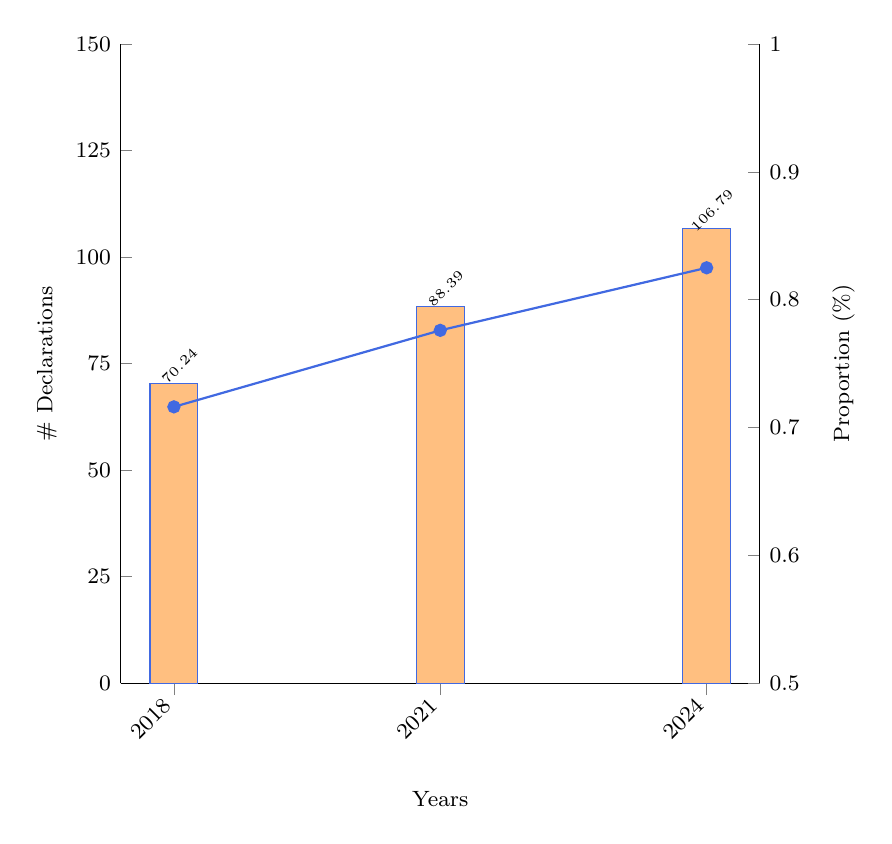
\begin{tikzpicture}
                    \begin{axis}[
    ybar,
    bar width=0.05\linewidth,
    width=0.8\textwidth,
    height=0.8\textwidth,
    xlabel={Years},
    x label style={anchor=north, below=1mm},
    ylabel={\#~Declarations},
    y label style={font=\footnotesize},
    ymin=0,
    ymax=150,
    ytick={0, 25, 50, 75, 100, 125, 150},
    y tick label style={font=\footnotesize},
    xtick={2015,2018,2021,2024},
    legend style={at={(0.5,-0.25)}, anchor=north, legend columns=2},
    x label style={anchor=south,yshift=-2em,font=\footnotesize},
    axis y line*=left,
    axis x line*=bottom,
    x tick label style={/pgf/number format/1000 sep=, rotate=45,anchor=east,font=\footnotesize},
    every node near coord/.style={/pgf/number format/1000 sep=, rotate=45, yshift=-0.2em, xshift=0.6em, font=\tiny},
    nodes near coords
]
    \addplot[fill=orange!50!white,draw=MyRoyalBlue,] coordinates {
       (2018, 70.24242424242425)
       (2021, 88.39393939393939)
       (2024, 106.78787878787878)
   };

\end{axis}

\begin{axis}[
    width=0.8\textwidth,
    height=0.8\textwidth,
    ymin=0.5,
    ymax=1,
    ytick={0.5, 0.6, 0.7, 0.8, 0.9, 1},
    y tick label style={font=\footnotesize},
    axis y line*=right,
    ylabel near ticks,
    yticklabel pos=right,
    ylabel={Proportion (\%)},
    axis x line=none,
    y label style={anchor=south, yshift=-2em, font=\footnotesize},
    legend style={at={(0,-0.35)}, anchor=north, legend columns=2}
]

    \addplot[MyRoyalBlue, thick, mark=*] coordinates {
       (2018, 0.7162229632371229)
       (2021, 0.7760622729720591)
       (2024, 0.8249854364915246)
   };

\end{axis}

                \end{tikzpicture}

                \\
                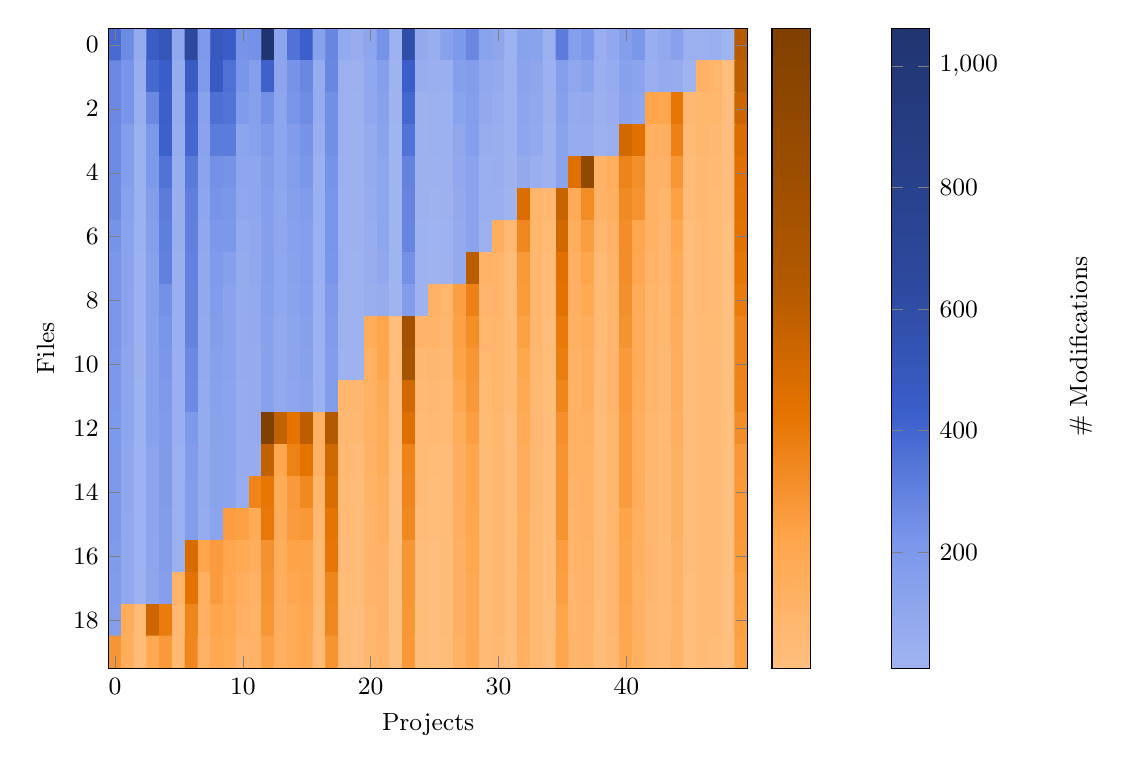
\begin{tikzpicture}
    \begin{axis}[
        enlargelimits=false,
        colorbar,
        colormap name=CustomBlue,
        colorbar shift/.style={xshift=0.15\textwidth},
        colorbar style={
            width=0.04\textwidth,
            title={\#~Modifications},     % Titre de la colorbar
            title style={font=\small,
            yshift=-0.35\textwidth,
            xshift=0.2\textwidth,
            rotate=90}, % Style du titre
        },
        width=0.8\textwidth,
        height=0.8\textwidth,
        xlabel=Projects,
        ylabel=Files,
        ylabel style={font=\small},
        xlabel style={font=\small},
        tick label style={font=\small},
    ]
        \addplot [matrix plot, point meta=explicit] coordinates {
(0,0) [385] (1,0) [259] (2,0) [71] (3,0) [453] (4,0) [520] (5,0) [92] (6,0) [646] (7,0) [188] (8,0) [481] (9,0) [452] (10,0) [226] (11,0) [233] (12,0) [1061] (13,0) [114] (14,0) [354] (15,0) [425] (16,0) [144] (17,0) [282] (18,0) [83] (19,0) [57] (20,0) [107] (21,0) [232] (22,0) [22] (23,0) [592] (24,0) [89] (25,0) [51] (26,0) [141] (27,0) [200] (28,0) [273] (29,0) [128] (30,0) [104] (31,0) [25] (32,0) [136] (33,0) [130] (34,0) [35] (35,0) [320] (36,0) [153] (37,0) [204] (38,0) [54] (39,0) [92] (40,0) [165] (41,0) [211] (42,0) [50] (43,0) [85] (44,0) [143] (45,0) [35] (46,0) [40] (47,0) [42] (48,0) [9] (49,0) [nan] 

(0,1) [270] (1,1) [224] (2,1) [49] (3,1) [391] (4,1) [435] (5,1) [69] (6,1) [459] (7,1) [185] (8,1) [464] (9,1) [363] (10,1) [219] (11,1) [158] (12,1) [419] (13,1) [111] (14,1) [231] (15,1) [271] (16,1) [64] (17,1) [277] (18,1) [38] (19,1) [39] (20,1) [96] (21,1) [155] (22,1) [16] (23,1) [437] (24,1) [57] (25,1) [44] (26,1) [47] (27,1) [153] (28,1) [167] (29,1) [90] (30,1) [76] (31,1) [25] (32,1) [125] (33,1) [105] (34,1) [31] (35,1) [161] (36,1) [97] (37,1) [134] (38,1) [45] (39,1) [67] (40,1) [144] (41,1) [122] (42,1) [41] (43,1) [69] (44,1) [67] (45,1) [18] (46,1) [nan] (47,1) [nan] (48,1) [nan] (49,1) [nan] 

(0,2) [268] (1,2) [222] (2,2) [41] (3,2) [270] (4,2) [424] (5,2) [65] (6,2) [406] (7,2) [136] (8,2) [365] (9,2) [347] (10,2) [182] (11,2) [151] (12,2) [237] (13,2) [107] (14,2) [223] (15,2) [256] (16,2) [63] (17,2) [247] (18,2) [37] (19,2) [33] (20,2) [93] (21,2) [143] (22,2) [13] (23,2) [401] (24,2) [28] (25,2) [39] (26,2) [33] (27,2) [130] (28,2) [160] (29,2) [83] (30,2) [56] (31,2) [24] (32,2) [117] (33,2) [93] (34,2) [27] (35,2) [152] (36,2) [69] (37,2) [81] (38,2) [37] (39,2) [60] (40,2) [127] (41,2) [108] (42,2) [nan] (43,2) [nan] (44,2) [nan] (45,2) [nan] (46,2) [nan] (47,2) [nan] (48,2) [nan] (49,2) [nan] 

(0,3) [261] (1,3) [166] (2,3) [38] (3,3) [206] (4,3) [420] (5,3) [58] (6,3) [395] (7,3) [126] (8,3) [318] (9,3) [319] (10,3) [115] (11,3) [141] (12,3) [191] (13,3) [106] (14,3) [176] (15,3) [230] (16,3) [53] (17,3) [246] (18,3) [37] (19,3) [32] (20,3) [71] (21,3) [126] (22,3) [12] (23,3) [351] (24,3) [27] (25,3) [35] (26,3) [29] (27,3) [99] (28,3) [156] (29,3) [57] (30,3) [51] (31,3) [23] (32,3) [106] (33,3) [85] (34,3) [26] (35,3) [131] (36,3) [65] (37,3) [63] (38,3) [27] (39,3) [42] (40,3) [nan] (41,3) [nan] (42,3) [nan] (43,3) [nan] (44,3) [nan] (45,3) [nan] (46,3) [nan] (47,3) [nan] (48,3) [nan] (49,3) [nan] 

(0,4) [261] (1,4) [164] (2,4) [37] (3,4) [201] (4,4) [355] (5,4) [52] (6,4) [324] (7,4) [120] (8,4) [240] (9,4) [231] (10,4) [109] (11,4) [109] (12,4) [168] (13,4) [106] (14,4) [164] (15,4) [215] (16,4) [40] (17,4) [229] (18,4) [34] (19,4) [30] (20,4) [69] (21,4) [110] (22,4) [11] (23,4) [293] (24,4) [27] (25,4) [32] (26,4) [27] (27,4) [91] (28,4) [127] (29,4) [47] (30,4) [50] (31,4) [20] (32,4) [89] (33,4) [45] (34,4) [25] (35,4) [128] (36,4) [nan] (37,4) [nan] (38,4) [nan] (39,4) [nan] (40,4) [nan] (41,4) [nan] (42,4) [nan] (43,4) [nan] (44,4) [nan] (45,4) [nan] (46,4) [nan] (47,4) [nan] (48,4) [nan] (49,4) [nan] 

(0,5) [259] (1,5) [143] (2,5) [35] (3,5) [169] (4,5) [320] (5,5) [51] (6,5) [305] (7,5) [107] (8,5) [227] (9,5) [212] (10,5) [98] (11,5) [107] (12,5) [158] (13,5) [102] (14,5) [149] (15,5) [179] (16,5) [40] (17,5) [222] (18,5) [32] (19,5) [28] (20,5) [67] (21,5) [109] (22,5) [11] (23,5) [287] (24,5) [27] (25,5) [21] (26,5) [27] (27,5) [88] (28,5) [126] (29,5) [42] (30,5) [46] (31,5) [18] (32,5) [nan] (33,5) [nan] (34,5) [nan] (35,5) [nan] (36,5) [nan] (37,5) [nan] (38,5) [nan] (39,5) [nan] (40,5) [nan] (41,5) [nan] (42,5) [nan] (43,5) [nan] (44,5) [nan] (45,5) [nan] (46,5) [nan] (47,5) [nan] (48,5) [nan] (49,5) [nan] 

(0,6) [232] (1,6) [129] (2,6) [34] (3,6) [159] (4,6) [307] (5,6) [48] (6,6) [303] (7,6) [93] (8,6) [204] (9,6) [206] (10,6) [80] (11,6) [97] (12,6) [157] (13,6) [99] (14,6) [142] (15,6) [166] (16,6) [38] (17,6) [222] (18,6) [30] (19,6) [27] (20,6) [59] (21,6) [106] (22,6) [11] (23,6) [279] (24,6) [24] (25,6) [16] (26,6) [26] (27,6) [81] (28,6) [126] (29,6) [37] (30,6) [nan] (31,6) [nan] (32,6) [nan] (33,6) [nan] (34,6) [nan] (35,6) [nan] (36,6) [nan] (37,6) [nan] (38,6) [nan] (39,6) [nan] (40,6) [nan] (41,6) [nan] (42,6) [nan] (43,6) [nan] (44,6) [nan] (45,6) [nan] (46,6) [nan] (47,6) [nan] (48,6) [nan] (49,6) [nan] 

(0,7) [210] (1,7) [125] (2,7) [33] (3,7) [150] (4,7) [298] (5,7) [46] (6,7) [294] (7,7) [87] (8,7) [186] (9,7) [150] (10,7) [75] (11,7) [97] (12,7) [155] (13,7) [96] (14,7) [137] (15,7) [160] (16,7) [38] (17,7) [219] (18,7) [29] (19,7) [26] (20,7) [58] (21,7) [93] (22,7) [11] (23,7) [239] (24,7) [22] (25,7) [15] (26,7) [21] (27,7) [79] (28,7) [nan] (29,7) [nan] (30,7) [nan] (31,7) [nan] (32,7) [nan] (33,7) [nan] (34,7) [nan] (35,7) [nan] (36,7) [nan] (37,7) [nan] (38,7) [nan] (39,7) [nan] (40,7) [nan] (41,7) [nan] (42,7) [nan] (43,7) [nan] (44,7) [nan] (45,7) [nan] (46,7) [nan] (47,7) [nan] (48,7) [nan] (49,7) [nan] 

(0,8) [210] (1,8) [120] (2,8) [33] (3,8) [146] (4,8) [238] (5,8) [44] (6,8) [293] (7,8) [83] (8,8) [180] (9,8) [125] (10,8) [74] (11,8) [82] (12,8) [151] (13,8) [96] (14,8) [126] (15,8) [158] (16,8) [32] (17,8) [189] (18,8) [27] (19,8) [25] (20,8) [53] (21,8) [67] (22,8) [10] (23,8) [168] (24,8) [20] (25,8) [nan] (26,8) [nan] (27,8) [nan] (28,8) [nan] (29,8) [nan] (30,8) [nan] (31,8) [nan] (32,8) [nan] (33,8) [nan] (34,8) [nan] (35,8) [nan] (36,8) [nan] (37,8) [nan] (38,8) [nan] (39,8) [nan] (40,8) [nan] (41,8) [nan] (42,8) [nan] (43,8) [nan] (44,8) [nan] (45,8) [nan] (46,8) [nan] (47,8) [nan] (48,8) [nan] (49,8) [nan] 

(0,9) [209] (1,9) [119] (2,9) [30] (3,9) [145] (4,9) [223] (5,9) [43] (6,9) [293] (7,9) [78] (8,9) [170] (9,9) [125] (10,9) [72] (11,9) [80] (12,9) [144] (13,9) [89] (14,9) [112] (15,9) [146] (16,9) [32] (17,9) [178] (18,9) [27] (19,9) [24] (20,9) [nan] (21,9) [nan] (22,9) [nan] (23,9) [nan] (24,9) [nan] (25,9) [nan] (26,9) [nan] (27,9) [nan] (28,9) [nan] (29,9) [nan] (30,9) [nan] (31,9) [nan] (32,9) [nan] (33,9) [nan] (34,9) [nan] (35,9) [nan] (36,9) [nan] (37,9) [nan] (38,9) [nan] (39,9) [nan] (40,9) [nan] (41,9) [nan] (42,9) [nan] (43,9) [nan] (44,9) [nan] (45,9) [nan] (46,9) [nan] (47,9) [nan] (48,9) [nan] (49,9) [nan] 

(0,10) [203] (1,10) [114] (2,10) [27] (3,10) [145] (4,10) [210] (5,10) [43] (6,10) [269] (7,10) [76] (8,10) [151] (9,10) [125] (10,10) [72] (11,10) [73] (12,10) [143] (13,10) [83] (14,10) [111] (15,10) [143] (16,10) [31] (17,10) [173] (18,10) [23] (19,10) [22] (20,10) [nan] (21,10) [nan] (22,10) [nan] (23,10) [nan] (24,10) [nan] (25,10) [nan] (26,10) [nan] (27,10) [nan] (28,10) [nan] (29,10) [nan] (30,10) [nan] (31,10) [nan] (32,10) [nan] (33,10) [nan] (34,10) [nan] (35,10) [nan] (36,10) [nan] (37,10) [nan] (38,10) [nan] (39,10) [nan] (40,10) [nan] (41,10) [nan] (42,10) [nan] (43,10) [nan] (44,10) [nan] (45,10) [nan] (46,10) [nan] (47,10) [nan] (48,10) [nan] (49,10) [nan] 

(0,11) [203] (1,11) [109] (2,11) [25] (3,11) [141] (4,11) [191] (5,11) [43] (6,11) [264] (7,11) [74] (8,11) [141] (9,11) [123] (10,11) [67] (11,11) [72] (12,11) [139] (13,11) [83] (14,11) [106] (15,11) [127] (16,11) [31] (17,11) [170] (18,11) [nan] (19,11) [nan] (20,11) [nan] (21,11) [nan] (22,11) [nan] (23,11) [nan] (24,11) [nan] (25,11) [nan] (26,11) [nan] (27,11) [nan] (28,11) [nan] (29,11) [nan] (30,11) [nan] (31,11) [nan] (32,11) [nan] (33,11) [nan] (34,11) [nan] (35,11) [nan] (36,11) [nan] (37,11) [nan] (38,11) [nan] (39,11) [nan] (40,11) [nan] (41,11) [nan] (42,11) [nan] (43,11) [nan] (44,11) [nan] (45,11) [nan] (46,11) [nan] (47,11) [nan] (48,11) [nan] (49,11) [nan] 

(0,12) [201] (1,12) [107] (2,12) [25] (3,12) [140] (4,12) [185] (5,12) [41] (6,12) [200] (7,12) [74] (8,12) [136] (9,12) [123] (10,12) [64] (11,12) [69] (12,12) [nan] (13,12) [nan] (14,12) [nan] (15,12) [nan] (16,12) [nan] (17,12) [nan] (18,12) [nan] (19,12) [nan] (20,12) [nan] (21,12) [nan] (22,12) [nan] (23,12) [nan] (24,12) [nan] (25,12) [nan] (26,12) [nan] (27,12) [nan] (28,12) [nan] (29,12) [nan] (30,12) [nan] (31,12) [nan] (32,12) [nan] (33,12) [nan] (34,12) [nan] (35,12) [nan] (36,12) [nan] (37,12) [nan] (38,12) [nan] (39,12) [nan] (40,12) [nan] (41,12) [nan] (42,12) [nan] (43,12) [nan] (44,12) [nan] (45,12) [nan] (46,12) [nan] (47,12) [nan] (48,12) [nan] (49,12) [nan] 

(0,13) [198] (1,13) [101] (2,13) [24] (3,13) [124] (4,13) [182] (5,13) [40] (6,13) [176] (7,13) [72] (8,13) [131] (9,13) [121] (10,13) [62] (11,13) [64] (12,13) [nan] (13,13) [nan] (14,13) [nan] (15,13) [nan] (16,13) [nan] (17,13) [nan] (18,13) [nan] (19,13) [nan] (20,13) [nan] (21,13) [nan] (22,13) [nan] (23,13) [nan] (24,13) [nan] (25,13) [nan] (26,13) [nan] (27,13) [nan] (28,13) [nan] (29,13) [nan] (30,13) [nan] (31,13) [nan] (32,13) [nan] (33,13) [nan] (34,13) [nan] (35,13) [nan] (36,13) [nan] (37,13) [nan] (38,13) [nan] (39,13) [nan] (40,13) [nan] (41,13) [nan] (42,13) [nan] (43,13) [nan] (44,13) [nan] (45,13) [nan] (46,13) [nan] (47,13) [nan] (48,13) [nan] (49,13) [nan] 

(0,14) [197] (1,14) [101] (2,14) [24] (3,14) [119] (4,14) [181] (5,14) [39] (6,14) [172] (7,14) [70] (8,14) [128] (9,14) [120] (10,14) [61] (11,14) [nan] (12,14) [nan] (13,14) [nan] (14,14) [nan] (15,14) [nan] (16,14) [nan] (17,14) [nan] (18,14) [nan] (19,14) [nan] (20,14) [nan] (21,14) [nan] (22,14) [nan] (23,14) [nan] (24,14) [nan] (25,14) [nan] (26,14) [nan] (27,14) [nan] (28,14) [nan] (29,14) [nan] (30,14) [nan] (31,14) [nan] (32,14) [nan] (33,14) [nan] (34,14) [nan] (35,14) [nan] (36,14) [nan] (37,14) [nan] (38,14) [nan] (39,14) [nan] (40,14) [nan] (41,14) [nan] (42,14) [nan] (43,14) [nan] (44,14) [nan] (45,14) [nan] (46,14) [nan] (47,14) [nan] (48,14) [nan] (49,14) [nan] 

(0,15) [196] (1,15) [94] (2,15) [24] (3,15) [119] (4,15) [173] (5,15) [38] (6,15) [171] (7,15) [66] (8,15) [120] (9,15) [nan] (10,15) [nan] (11,15) [nan] (12,15) [nan] (13,15) [nan] (14,15) [nan] (15,15) [nan] (16,15) [nan] (17,15) [nan] (18,15) [nan] (19,15) [nan] (20,15) [nan] (21,15) [nan] (22,15) [nan] (23,15) [nan] (24,15) [nan] (25,15) [nan] (26,15) [nan] (27,15) [nan] (28,15) [nan] (29,15) [nan] (30,15) [nan] (31,15) [nan] (32,15) [nan] (33,15) [nan] (34,15) [nan] (35,15) [nan] (36,15) [nan] (37,15) [nan] (38,15) [nan] (39,15) [nan] (40,15) [nan] (41,15) [nan] (42,15) [nan] (43,15) [nan] (44,15) [nan] (45,15) [nan] (46,15) [nan] (47,15) [nan] (48,15) [nan] (49,15) [nan] 

(0,16) [183] (1,16) [93] (2,16) [23] (3,16) [117] (4,16) [167] (5,16) [37] (6,16) [nan] (7,16) [nan] (8,16) [nan] (9,16) [nan] (10,16) [nan] (11,16) [nan] (12,16) [nan] (13,16) [nan] (14,16) [nan] (15,16) [nan] (16,16) [nan] (17,16) [nan] (18,16) [nan] (19,16) [nan] (20,16) [nan] (21,16) [nan] (22,16) [nan] (23,16) [nan] (24,16) [nan] (25,16) [nan] (26,16) [nan] (27,16) [nan] (28,16) [nan] (29,16) [nan] (30,16) [nan] (31,16) [nan] (32,16) [nan] (33,16) [nan] (34,16) [nan] (35,16) [nan] (36,16) [nan] (37,16) [nan] (38,16) [nan] (39,16) [nan] (40,16) [nan] (41,16) [nan] (42,16) [nan] (43,16) [nan] (44,16) [nan] (45,16) [nan] (46,16) [nan] (47,16) [nan] (48,16) [nan] (49,16) [nan] 

(0,17) [175] (1,17) [93] (2,17) [22] (3,17) [104] (4,17) [166] (5,17) [nan] (6,17) [nan] (7,17) [nan] (8,17) [nan] (9,17) [nan] (10,17) [nan] (11,17) [nan] (12,17) [nan] (13,17) [nan] (14,17) [nan] (15,17) [nan] (16,17) [nan] (17,17) [nan] (18,17) [nan] (19,17) [nan] (20,17) [nan] (21,17) [nan] (22,17) [nan] (23,17) [nan] (24,17) [nan] (25,17) [nan] (26,17) [nan] (27,17) [nan] (28,17) [nan] (29,17) [nan] (30,17) [nan] (31,17) [nan] (32,17) [nan] (33,17) [nan] (34,17) [nan] (35,17) [nan] (36,17) [nan] (37,17) [nan] (38,17) [nan] (39,17) [nan] (40,17) [nan] (41,17) [nan] (42,17) [nan] (43,17) [nan] (44,17) [nan] (45,17) [nan] (46,17) [nan] (47,17) [nan] (48,17) [nan] (49,17) [nan] 

(0,18) [165] (1,18) [nan] (2,18) [nan] (3,18) [nan] (4,18) [nan] (5,18) [nan] (6,18) [nan] (7,18) [nan] (8,18) [nan] (9,18) [nan] (10,18) [nan] (11,18) [nan] (12,18) [nan] (13,18) [nan] (14,18) [nan] (15,18) [nan] (16,18) [nan] (17,18) [nan] (18,18) [nan] (19,18) [nan] (20,18) [nan] (21,18) [nan] (22,18) [nan] (23,18) [nan] (24,18) [nan] (25,18) [nan] (26,18) [nan] (27,18) [nan] (28,18) [nan] (29,18) [nan] (30,18) [nan] (31,18) [nan] (32,18) [nan] (33,18) [nan] (34,18) [nan] (35,18) [nan] (36,18) [nan] (37,18) [nan] (38,18) [nan] (39,18) [nan] (40,18) [nan] (41,18) [nan] (42,18) [nan] (43,18) [nan] (44,18) [nan] (45,18) [nan] (46,18) [nan] (47,18) [nan] (48,18) [nan] (49,18) [nan] 

(0,19) [nan] (1,19) [nan] (2,19) [nan] (3,19) [nan] (4,19) [nan] (5,19) [nan] (6,19) [nan] (7,19) [nan] (8,19) [nan] (9,19) [nan] (10,19) [nan] (11,19) [nan] (12,19) [nan] (13,19) [nan] (14,19) [nan] (15,19) [nan] (16,19) [nan] (17,19) [nan] (18,19) [nan] (19,19) [nan] (20,19) [nan] (21,19) [nan] (22,19) [nan] (23,19) [nan] (24,19) [nan] (25,19) [nan] (26,19) [nan] (27,19) [nan] (28,19) [nan] (29,19) [nan] (30,19) [nan] (31,19) [nan] (32,19) [nan] (33,19) [nan] (34,19) [nan] (35,19) [nan] (36,19) [nan] (37,19) [nan] (38,19) [nan] (39,19) [nan] (40,19) [nan] (41,19) [nan] (42,19) [nan] (43,19) [nan] (44,19) [nan] (45,19) [nan] (46,19) [nan] (47,19) [nan] (48,19) [nan] (49,19) [nan] 

};

    \end{axis}
    \begin{axis}[
        enlargelimits=false,
        colorbar,
        colormap name=CustomOrange,
        colorbar style={width=0.04\textwidth, ytick=\empty},
        width=0.8\textwidth,
        height=0.8\textwidth,
        ylabel=\empty,
        xlabel=\empty,
        yticklabel=\empty,
        xticklabel=\empty
    ]
        \addplot [matrix plot, point meta=explicit] coordinates {
(0,0) [nan] (1,0) [nan] (2,0) [nan] (3,0) [nan] (4,0) [nan] (5,0) [nan] (6,0) [nan] (7,0) [nan] (8,0) [nan] (9,0) [nan] (10,0) [nan] (11,0) [nan] (12,0) [nan] (13,0) [nan] (14,0) [nan] (15,0) [nan] (16,0) [nan] (17,0) [nan] (18,0) [nan] (19,0) [nan] (20,0) [nan] (21,0) [nan] (22,0) [nan] (23,0) [nan] (24,0) [nan] (25,0) [nan] (26,0) [nan] (27,0) [nan] (28,0) [nan] (29,0) [nan] (30,0) [nan] (31,0) [nan] (32,0) [nan] (33,0) [nan] (34,0) [nan] (35,0) [nan] (36,0) [nan] (37,0) [nan] (38,0) [nan] (39,0) [nan] (40,0) [nan] (41,0) [nan] (42,0) [nan] (43,0) [nan] (44,0) [nan] (45,0) [nan] (46,0) [nan] (47,0) [nan] (48,0) [nan] (49,0) [374] 

(0,1) [nan] (1,1) [nan] (2,1) [nan] (3,1) [nan] (4,1) [nan] (5,1) [nan] (6,1) [nan] (7,1) [nan] (8,1) [nan] (9,1) [nan] (10,1) [nan] (11,1) [nan] (12,1) [nan] (13,1) [nan] (14,1) [nan] (15,1) [nan] (16,1) [nan] (17,1) [nan] (18,1) [nan] (19,1) [nan] (20,1) [nan] (21,1) [nan] (22,1) [nan] (23,1) [nan] (24,1) [nan] (25,1) [nan] (26,1) [nan] (27,1) [nan] (28,1) [nan] (29,1) [nan] (30,1) [nan] (31,1) [nan] (32,1) [nan] (33,1) [nan] (34,1) [nan] (35,1) [nan] (36,1) [nan] (37,1) [nan] (38,1) [nan] (39,1) [nan] (40,1) [nan] (41,1) [nan] (42,1) [nan] (43,1) [nan] (44,1) [nan] (45,1) [nan] (46,1) [73] (47,1) [56] (48,1) [13] (49,1) [350] 

(0,2) [nan] (1,2) [nan] (2,2) [nan] (3,2) [nan] (4,2) [nan] (5,2) [nan] (6,2) [nan] (7,2) [nan] (8,2) [nan] (9,2) [nan] (10,2) [nan] (11,2) [nan] (12,2) [nan] (13,2) [nan] (14,2) [nan] (15,2) [nan] (16,2) [nan] (17,2) [nan] (18,2) [nan] (19,2) [nan] (20,2) [nan] (21,2) [nan] (22,2) [nan] (23,2) [nan] (24,2) [nan] (25,2) [nan] (26,2) [nan] (27,2) [nan] (28,2) [nan] (29,2) [nan] (30,2) [nan] (31,2) [nan] (32,2) [nan] (33,2) [nan] (34,2) [nan] (35,2) [nan] (36,2) [nan] (37,2) [nan] (38,2) [nan] (39,2) [nan] (40,2) [nan] (41,2) [nan] (42,2) [131] (43,2) [128] (44,2) [249] (45,2) [42] (46,2) [53] (47,2) [53] (48,2) [12] (49,2) [321] 

(0,3) [nan] (1,3) [nan] (2,3) [nan] (3,3) [nan] (4,3) [nan] (5,3) [nan] (6,3) [nan] (7,3) [nan] (8,3) [nan] (9,3) [nan] (10,3) [nan] (11,3) [nan] (12,3) [nan] (13,3) [nan] (14,3) [nan] (15,3) [nan] (16,3) [nan] (17,3) [nan] (18,3) [nan] (19,3) [nan] (20,3) [nan] (21,3) [nan] (22,3) [nan] (23,3) [nan] (24,3) [nan] (25,3) [nan] (26,3) [nan] (27,3) [nan] (28,3) [nan] (29,3) [nan] (30,3) [nan] (31,3) [nan] (32,3) [nan] (33,3) [nan] (34,3) [nan] (35,3) [nan] (36,3) [nan] (37,3) [nan] (38,3) [nan] (39,3) [nan] (40,3) [308] (41,3) [268] (42,3) [82] (43,3) [86] (44,3) [222] (45,3) [30] (46,3) [48] (47,3) [41] (48,3) [12] (49,3) [282] 

(0,4) [nan] (1,4) [nan] (2,4) [nan] (3,4) [nan] (4,4) [nan] (5,4) [nan] (6,4) [nan] (7,4) [nan] (8,4) [nan] (9,4) [nan] (10,4) [nan] (11,4) [nan] (12,4) [nan] (13,4) [nan] (14,4) [nan] (15,4) [nan] (16,4) [nan] (17,4) [nan] (18,4) [nan] (19,4) [nan] (20,4) [nan] (21,4) [nan] (22,4) [nan] (23,4) [nan] (24,4) [nan] (25,4) [nan] (26,4) [nan] (27,4) [nan] (28,4) [nan] (29,4) [nan] (30,4) [nan] (31,4) [nan] (32,4) [nan] (33,4) [nan] (34,4) [nan] (35,4) [nan] (36,4) [271] (37,4) [547] (38,4) [67] (39,4) [91] (40,4) [217] (41,4) [186] (42,4) [73] (43,4) [72] (44,4) [172] (45,4) [27] (46,4) [43] (47,4) [39] (48,4) [12] (49,4) [269] 

(0,5) [nan] (1,5) [nan] (2,5) [nan] (3,5) [nan] (4,5) [nan] (5,5) [nan] (6,5) [nan] (7,5) [nan] (8,5) [nan] (9,5) [nan] (10,5) [nan] (11,5) [nan] (12,5) [nan] (13,5) [nan] (14,5) [nan] (15,5) [nan] (16,5) [nan] (17,5) [nan] (18,5) [nan] (19,5) [nan] (20,5) [nan] (21,5) [nan] (22,5) [nan] (23,5) [nan] (24,5) [nan] (25,5) [nan] (26,5) [nan] (27,5) [nan] (28,5) [nan] (29,5) [nan] (30,5) [nan] (31,5) [nan] (32,5) [280] (33,5) [55] (34,5) [43] (35,5) [329] (36,5) [108] (37,5) [196] (38,5) [66] (39,5) [86] (40,5) [201] (41,5) [175] (42,5) [71] (43,5) [60] (44,5) [147] (45,5) [24] (46,5) [41] (47,5) [36] (48,5) [12] (49,5) [267] 

(0,6) [nan] (1,6) [nan] (2,6) [nan] (3,6) [nan] (4,6) [nan] (5,6) [nan] (6,6) [nan] (7,6) [nan] (8,6) [nan] (9,6) [nan] (10,6) [nan] (11,6) [nan] (12,6) [nan] (13,6) [nan] (14,6) [nan] (15,6) [nan] (16,6) [nan] (17,6) [nan] (18,6) [nan] (19,6) [nan] (20,6) [nan] (21,6) [nan] (22,6) [nan] (23,6) [nan] (24,6) [nan] (25,6) [nan] (26,6) [nan] (27,6) [nan] (28,6) [nan] (29,6) [nan] (30,6) [91] (31,6) [39] (32,6) [206] (33,6) [53] (34,6) [35] (35,6) [311] (36,6) [91] (37,6) [153] (38,6) [47] (39,6) [71] (40,6) [193] (41,6) [127] (42,6) [71] (43,6) [47] (44,6) [121] (45,6) [22] (46,6) [38] (47,6) [36] (48,6) [10] (49,6) [262] 

(0,7) [nan] (1,7) [nan] (2,7) [nan] (3,7) [nan] (4,7) [nan] (5,7) [nan] (6,7) [nan] (7,7) [nan] (8,7) [nan] (9,7) [nan] (10,7) [nan] (11,7) [nan] (12,7) [nan] (13,7) [nan] (14,7) [nan] (15,7) [nan] (16,7) [nan] (17,7) [nan] (18,7) [nan] (19,7) [nan] (20,7) [nan] (21,7) [nan] (22,7) [nan] (23,7) [nan] (24,7) [nan] (25,7) [nan] (26,7) [nan] (27,7) [nan] (28,7) [363] (29,7) [68] (30,7) [64] (31,7) [25] (32,7) [162] (33,7) [51] (34,7) [28] (35,7) [269] (36,7) [80] (37,7) [133] (38,7) [34] (39,7) [62] (40,7) [192] (41,7) [120] (42,7) [63] (43,7) [46] (44,7) [109] (45,7) [20] (46,7) [37] (47,7) [36] (48,7) [10] (49,7) [250] 

(0,8) [nan] (1,8) [nan] (2,8) [nan] (3,8) [nan] (4,8) [nan] (5,8) [nan] (6,8) [nan] (7,8) [nan] (8,8) [nan] (9,8) [nan] (10,8) [nan] (11,8) [nan] (12,8) [nan] (13,8) [nan] (14,8) [nan] (15,8) [nan] (16,8) [nan] (17,8) [nan] (18,8) [nan] (19,8) [nan] (20,8) [nan] (21,8) [nan] (22,8) [nan] (23,8) [nan] (24,8) [nan] (25,8) [71] (26,8) [56] (27,8) [150] (28,8) [222] (29,8) [56] (30,8) [63] (31,8) [24] (32,8) [159] (33,8) [48] (34,8) [26] (35,8) [261] (36,8) [80] (37,8) [118] (38,8) [32] (39,8) [57] (40,8) [185] (41,8) [103] (42,8) [60] (43,8) [45] (44,8) [103] (45,8) [19] (46,8) [37] (47,8) [35] (48,8) [10] (49,8) [235] 

(0,9) [nan] (1,9) [nan] (2,9) [nan] (3,9) [nan] (4,9) [nan] (5,9) [nan] (6,9) [nan] (7,9) [nan] (8,9) [nan] (9,9) [nan] (10,9) [nan] (11,9) [nan] (12,9) [nan] (13,9) [nan] (14,9) [nan] (15,9) [nan] (16,9) [nan] (17,9) [nan] (18,9) [nan] (19,9) [nan] (20,9) [97] (21,9) [134] (22,9) [13] (23,9) [464] (24,9) [62] (25,9) [62] (26,9) [47] (27,9) [143] (28,9) [190] (29,9) [49] (30,9) [58] (31,9) [23] (32,9) [144] (33,9) [46] (34,9) [22] (35,9) [240] (36,9) [79] (37,9) [99] (38,9) [31] (39,9) [56] (40,9) [179] (41,9) [102] (42,9) [58] (43,9) [45] (44,9) [99] (45,9) [19] (46,9) [36] (47,9) [35] (48,9) [10] (49,9) [217] 

(0,10) [nan] (1,10) [nan] (2,10) [nan] (3,10) [nan] (4,10) [nan] (5,10) [nan] (6,10) [nan] (7,10) [nan] (8,10) [nan] (9,10) [nan] (10,10) [nan] (11,10) [nan] (12,10) [nan] (13,10) [nan] (14,10) [nan] (15,10) [nan] (16,10) [nan] (17,10) [nan] (18,10) [nan] (19,10) [nan] (20,10) [74] (21,10) [131] (22,10) [13] (23,10) [436] (24,10) [42] (25,10) [47] (26,10) [44] (27,10) [140] (28,10) [170] (29,10) [40] (30,10) [57] (31,10) [23] (32,10) [126] (33,10) [42] (34,10) [21] (35,10) [229] (36,10) [76] (37,10) [93] (38,10) [28] (39,10) [56] (40,10) [164] (41,10) [100] (42,10) [58] (43,10) [43] (44,10) [92] (45,10) [19] (46,10) [34] (47,10) [34] (48,10) [9] (49,10) [217] 

(0,11) [nan] (1,11) [nan] (2,11) [nan] (3,11) [nan] (4,11) [nan] (5,11) [nan] (6,11) [nan] (7,11) [nan] (8,11) [nan] (9,11) [nan] (10,11) [nan] (11,11) [nan] (12,11) [nan] (13,11) [nan] (14,11) [nan] (15,11) [nan] (16,11) [nan] (17,11) [nan] (18,11) [50] (19,11) [49] (20,11) [74] (21,11) [109] (22,11) [12] (23,11) [304] (24,11) [37] (25,11) [41] (26,11) [32] (27,11) [120] (28,11) [165] (29,11) [35] (30,11) [56] (31,11) [23] (32,11) [115] (33,11) [42] (34,11) [21] (35,11) [211] (36,11) [76] (37,11) [91] (38,11) [27] (39,11) [55] (40,11) [163] (41,11) [98] (42,11) [55] (43,11) [42] (44,11) [91] (45,11) [18] (46,11) [34] (47,11) [33] (48,11) [9] (49,11) [215] 

(0,12) [nan] (1,12) [nan] (2,12) [nan] (3,12) [nan] (4,12) [nan] (5,12) [nan] (6,12) [nan] (7,12) [nan] (8,12) [nan] (9,12) [nan] (10,12) [nan] (11,12) [nan] (12,12) [631] (13,12) [341] (14,12) [257] (15,12) [359] (16,12) [76] (17,12) [386] (18,12) [44] (19,12) [42] (20,12) [74] (21,12) [106] (22,12) [12] (23,12) [275] (24,12) [34] (25,12) [40] (26,12) [32] (27,12) [98] (28,12) [149] (29,12) [35] (30,12) [53] (31,12) [22] (32,12) [109] (33,12) [42] (34,12) [20] (35,12) [187] (36,12) [74] (37,12) [82] (38,12) [27] (39,12) [53] (40,12) [159] (41,12) [93] (42,12) [53] (43,12) [38] (44,12) [86] (45,12) [18] (46,12) [34] (47,12) [33] (48,12) [9] (49,12) [194] 

(0,13) [nan] (1,13) [nan] (2,13) [nan] (3,13) [nan] (4,13) [nan] (5,13) [nan] (6,13) [nan] (7,13) [nan] (8,13) [nan] (9,13) [nan] (10,13) [nan] (11,13) [nan] (12,13) [343] (13,13) [128] (14,13) [219] (15,13) [258] (16,13) [73] (17,13) [309] (18,13) [40] (19,13) [28] (20,13) [69] (21,13) [103] (22,13) [11] (23,13) [216] (24,13) [34] (25,13) [26] (26,13) [27] (27,13) [88] (28,13) [134] (29,13) [34] (30,13) [51] (31,13) [22] (32,13) [99] (33,13) [42] (34,13) [20] (35,13) [176] (36,13) [74] (37,13) [76] (38,13) [24] (39,13) [52] (40,13) [157] (41,13) [91] (42,13) [53] (43,13) [36] (44,13) [79] (45,13) [18] (46,13) [33] (47,13) [33] (48,13) [9] (49,13) [166] 

(0,14) [nan] (1,14) [nan] (2,14) [nan] (3,14) [nan] (4,14) [nan] (5,14) [nan] (6,14) [nan] (7,14) [nan] (8,14) [nan] (9,14) [nan] (10,14) [nan] (11,14) [215] (12,14) [249] (13,14) [102] (14,14) [162] (15,14) [203] (16,14) [54] (17,14) [284] (18,14) [34] (19,14) [26] (20,14) [68] (21,14) [86] (22,14) [10] (23,14) [212] (24,14) [32] (25,14) [20] (26,14) [27] (27,14) [87] (28,14) [134] (29,14) [33] (30,14) [48] (31,14) [21] (32,14) [95] (33,14) [42] (34,14) [19] (35,14) [176] (36,14) [66] (37,14) [75] (38,14) [24] (39,14) [52] (40,14) [156] (41,14) [90] (42,14) [49] (43,14) [35] (44,14) [78] (45,14) [18] (46,14) [33] (47,14) [32] (48,14) [9] (49,14) [164] 

(0,15) [nan] (1,15) [nan] (2,15) [nan] (3,15) [nan] (4,15) [nan] (5,15) [nan] (6,15) [nan] (7,15) [nan] (8,15) [nan] (9,15) [153] (10,15) [146] (11,15) [104] (12,15) [243] (13,15) [100] (14,15) [158] (15,15) [167] (16,15) [45] (17,15) [255] (18,15) [31] (19,15) [25] (20,15) [64] (21,15) [85] (22,15) [10] (23,15) [203] (24,15) [24] (25,15) [17] (26,15) [24] (27,15) [85] (28,15) [129] (29,15) [33] (30,15) [48] (31,15) [21] (32,15) [94] (33,15) [42] (34,15) [19] (35,15) [175] (36,15) [63] (37,15) [72] (38,15) [24] (39,15) [49] (40,15) [140] (41,15) [89] (42,15) [49] (43,15) [35] (44,15) [77] (45,15) [17] (46,15) [32] (47,15) [32] (48,15) [9] (49,15) [163] 

(0,16) [nan] (1,16) [nan] (2,16) [nan] (3,16) [nan] (4,16) [nan] (5,16) [nan] (6,16) [292] (7,16) [131] (8,16) [156] (9,16) [130] (10,16) [113] (11,16) [90] (12,16) [181] (13,16) [94] (14,16) [140] (15,16) [139] (16,16) [40] (17,16) [248] (18,16) [28] (19,16) [25] (20,16) [63] (21,16) [73] (22,16) [10] (23,16) [172] (24,16) [22] (25,16) [15] (26,16) [24] (27,16) [82] (28,16) [128] (29,16) [33] (30,16) [48] (31,16) [20] (32,16) [93] (33,16) [42] (34,16) [18] (35,16) [153] (36,16) [61] (37,16) [68] (38,16) [24] (39,16) [48] (40,16) [136] (41,16) [86] (42,16) [48] (43,16) [33] (44,16) [70] (45,16) [17] (46,16) [31] (47,16) [32] (48,16) [8] (49,16) [161] 

(0,17) [nan] (1,17) [nan] (2,17) [nan] (3,17) [nan] (4,17) [nan] (5,17) [63] (6,17) [262] (7,17) [82] (8,17) [156] (9,17) [122] (10,17) [92] (11,17) [72] (12,17) [177] (13,17) [93] (14,17) [124] (15,17) [135] (16,17) [38] (17,17) [211] (18,17) [27] (19,17) [23] (20,17) [62] (21,17) [70] (22,17) [10] (23,17) [171] (24,17) [22] (25,17) [15] (26,17) [23] (27,17) [82] (28,17) [117] (29,17) [33] (30,17) [47] (31,17) [19] (32,17) [89] (33,17) [42] (34,17) [18] (35,17) [150] (36,17) [59] (37,17) [66] (38,17) [23] (39,17) [47] (40,17) [136] (41,17) [83] (42,17) [48] (43,17) [32] (44,17) [69] (45,17) [16] (46,17) [31] (47,17) [31] (48,17) [8] (49,17) [150] 

(0,18) [nan] (1,18) [98] (2,18) [28] (3,18) [318] (4,18) [234] (5,18) [41] (6,18) [211] (7,18) [78] (8,18) [132] (9,18) [119] (10,18) [81] (11,18) [70] (12,18) [171] (13,18) [88] (14,18) [114] (15,18) [130] (16,18) [35] (17,18) [205] (18,18) [24] (19,18) [22] (20,18) [54] (21,18) [66] (22,18) [10] (23,18) [169] (24,18) [21] (25,18) [14] (26,18) [23] (27,18) [82] (28,18) [117] (29,18) [32] (30,18) [46] (31,18) [19] (32,18) [88] (33,18) [42] (34,18) [17] (35,18) [131] (36,18) [55] (37,18) [64] (38,18) [23] (39,18) [47] (40,18) [129] (41,18) [81] (42,18) [41] (43,18) [32] (44,18) [65] (45,18) [16] (46,18) [30] (47,18) [30] (48,18) [8] (49,18) [146] 

(0,19) [174] (1,19) [94] (2,19) [23] (3,19) [119] (4,19) [163] (5,19) [40] (6,19) [208] (7,19) [72] (8,19) [120] (9,19) [113] (10,19) [64] (11,19) [67] (12,19) [143] (13,19) [86] (14,19) [112] (15,19) [127] (16,19) [34] (17,19) [177] (18,19) [24] (19,19) [22] (20,19) [50] (21,19) [61] (22,19) [10] (23,19) [167] (24,19) [20] (25,19) [14] (26,19) [21] (27,19) [74] (28,19) [117] (29,19) [32] (30,19) [43] (31,19) [18] (32,19) [84] (33,19) [41] (34,19) [17] (35,19) [131] (36,19) [55] (37,19) [64] (38,19) [23] (39,19) [42] (40,19) [128] (41,19) [79] (42,19) [41] (43,19) [32] (44,19) [64] (45,19) [16] (46,19) [30] (47,19) [28] (48,19) [8] (49,19) [141] 

};

    \end{axis}
\end{tikzpicture}

            \end{tabular}
        \end{minipage}
        \caption{
            Number of declarations of shared objects in the ASF projects:
            \emph{(top)} on average over time, and
            \emph{(bot)} in the 20 most modified files for the latest version of each project.
        }
    \end{figure}

    \begin{figure}
        \begin{tabular}{@{}l@{~~}l@{}}

  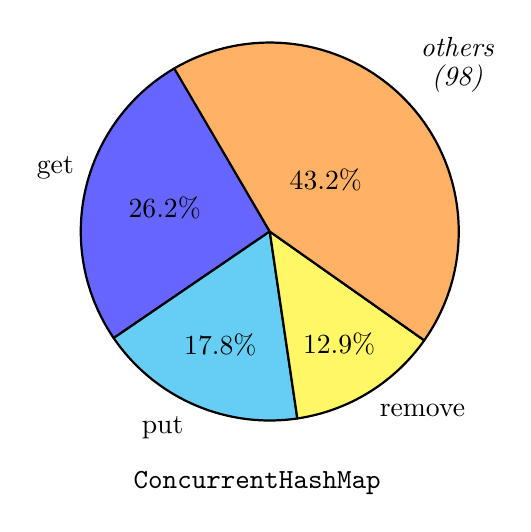
\begin{tikzpicture}[scale=0.8]
    \def\printonlylargeenough#1#2{\unless\ifdim#2pt<#1pt\relax
      #2\printnumbertrue
      \else
      \printnumberfalse
      \fi}
    \newif\ifprintnumber
    \pie[rotate=120, radius=3, before number=\printonlylargeenough{10}, after number=\ifprintnumber\%\fi]{26.2/\normalsize get, 17.8/\normalsize put, 12.9/\normalsize remove, 43.2/\normalsize \textit{\shortstack[c]{others\\(98)}}}
    \node () at (-.2,-4) {\bf\normalsize\code{ConcurrentHashMap}};
  \end{tikzpicture}

  &

  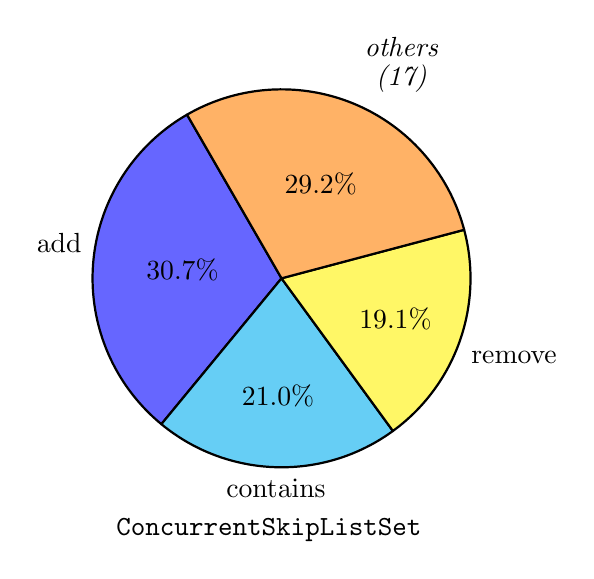
\begin{tikzpicture}[scale=0.8]
    \def\printonlylargeenough#1#2{\unless\ifdim#2pt<#1pt\relax
      #2\printnumbertrue
      \else
      \printnumberfalse
      \fi}
    \newif\ifprintnumber
    \pie[rotate=120, radius=3, before number=\printonlylargeenough{10}, after number=\ifprintnumber\%\fi]{30.7/\normalsize add, 21.0/\normalsize contains, 19.1/\normalsize remove, 29.2/\normalsize \textit{\shortstack[c]{others\\(17)}}}
    \node () at (-.2,-4) {\bf\normalsize\code{ConcurrentSkipListSet}};
  \end{tikzpicture}
\\

  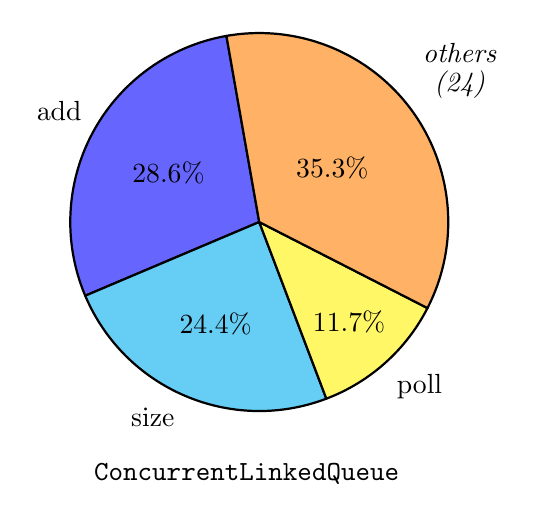
\begin{tikzpicture}[scale=0.8]
    \def\printonlylargeenough#1#2{\unless\ifdim#2pt<#1pt\relax
      #2\printnumbertrue
      \else
      \printnumberfalse
      \fi}
    \newif\ifprintnumber
    \pie[rotate=100, radius=3, before number=\printonlylargeenough{10}, after number=\ifprintnumber\%\fi]{28.6/\normalsize add, 24.4/\normalsize size, 11.7/\normalsize poll, 35.3/\normalsize \textit{\shortstack[c]{others\\(24)}}}
    \node () at (-.2,-4) {\bf\normalsize\code{ConcurrentLinkedQueue}};
  \end{tikzpicture}

  &

  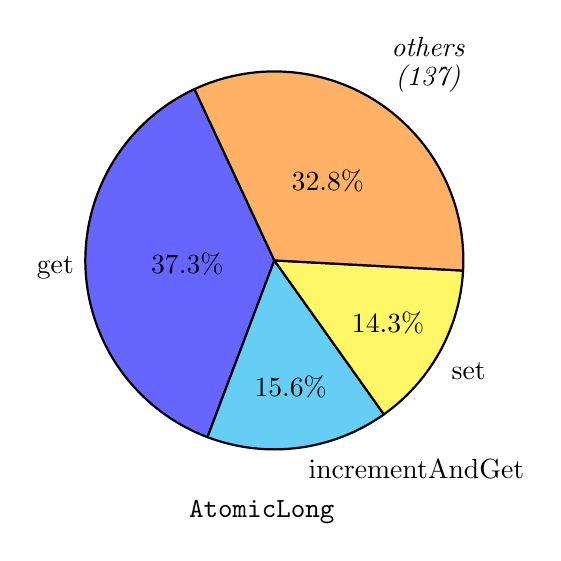
\begin{tikzpicture}[scale=0.8]
    \def\printonlylargeenough#1#2{\unless\ifdim#2pt<#1pt\relax
      #2\printnumbertrue
      \else
      \printnumberfalse
      \fi}
    \newif\ifprintnumber
    \pie[rotate=115, radius=3, before number=\printonlylargeenough{10}, after number=\ifprintnumber\%\fi]{37.3/\normalsize get, 15.6/\normalsize incrementAndGet, 14.3/\normalsize set, 32.8/\normalsize \textit{\shortstack[c]{others\\(137)}}}
    \node () at (-.2,-4) {\bf\normalsize\code{AtomicLong}};
  \end{tikzpicture}

\end{tabular}

        \caption{
            Most used methods in the ASF projects.
        }
    \end{figure}

    \begin{figure}
        \hspace{-10.8em}%
        \begin{tabular}[t]{c c c}
            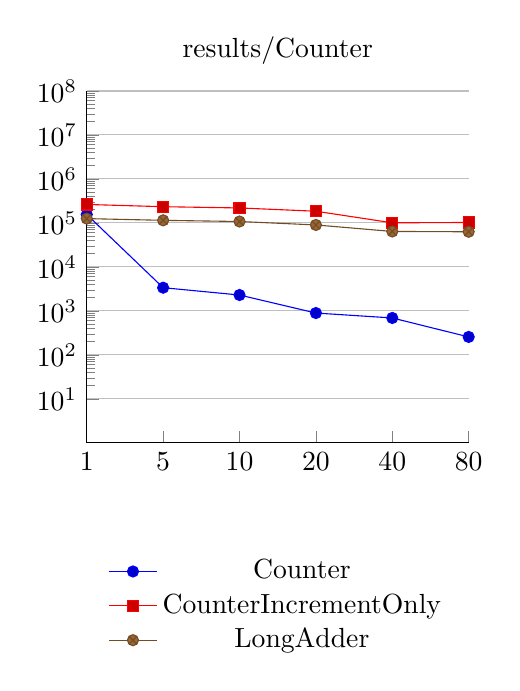
\begin{tikzpicture}[baseline={(current axis.north)}]
            \begin{axis}[
    xticklabels={1,5,10,20,40,80},
    xtick={1,2,3,4,5,6},
    ytick={0,10,1.0E2,1.0E3,1.0E4,1.0E5,1.0E6,1.0E7,1.0E8,1.0E9,1.0E10,1.0E11},
    ymin=1,
    ymax=100000000,
    xmin=1,
    xmax=6,
    y=0.02\textwidth,
    x=0.08\textwidth,
    ymode=log,
    log origin=0,
    ymajorgrids,
    axis x line*=bottom,
    axis y line*=left,
    ylabel style={font=\normalsize},
    xlabel style={font=\normalsize},
    title style={font=\normalsize},
    tick label style={font=\normalsize},
    legend style={draw=none, at={(0.5,-0.3)}, anchor=north,font=\normalsize},
    title=results/Counter]
    \addplot coordinates {
       (1, 154954)
       (2, 3361)
       (3, 2290)
       (4, 891)
       (5, 689)
       (6, 255)
   };

    \addplot coordinates {
       (1, 262569)
       (2, 233363)
       (3, 218526)
       (4, 184189)
       (5, 100354)
       (6, 102128)
   };

    \addplot coordinates {
       (1, 125094)
       (2, 114292)
       (3, 107447)
       (4, 89728)
       (5, 63816)
       (6, 62834)
   };

  \legend{Counter, CounterIncrementOnly, LongAdder, };
\end{axis}
            \end{tikzpicture}
            &
            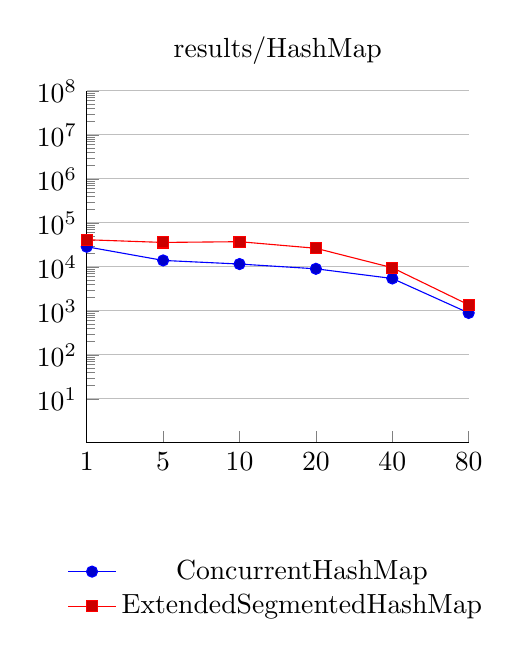
\begin{tikzpicture}[baseline={(current axis.north)}]
            \begin{axis}[
    xticklabels={1,5,10,20,40,80},
    xtick={1,2,3,4,5,6},
    ytick={0,10,1.0E2,1.0E3,1.0E4,1.0E5,1.0E6,1.0E7,1.0E8,1.0E9,1.0E10,1.0E11},
    ymin=1,
    ymax=100000000,
    xmin=1,
    xmax=6,
    y=0.02\textwidth,
    x=0.08\textwidth,
    ymode=log,
    log origin=0,
    ymajorgrids,
    axis x line*=bottom,
    axis y line*=left,
    ylabel style={font=\normalsize},
    xlabel style={font=\normalsize},
    title style={font=\normalsize},
    tick label style={font=\normalsize},
    legend style={draw=none, at={(0.5,-0.3)}, anchor=north,font=\normalsize},
    title=results/HashMap]
    \addplot coordinates {
       (1, 28632)
       (2, 14003)
       (3, 11587)
       (4, 9030)
       (5, 5444)
       (6, 895)
   };

    \addplot coordinates {
       (1, 41347)
       (2, 35924)
       (3, 37349)
       (4, 26451)
       (5, 9556)
       (6, 1370)
   };

  \legend{ConcurrentHashMap, ExtendedSegmentedHashMap, };
\end{axis}
            \end{tikzpicture}
            &
            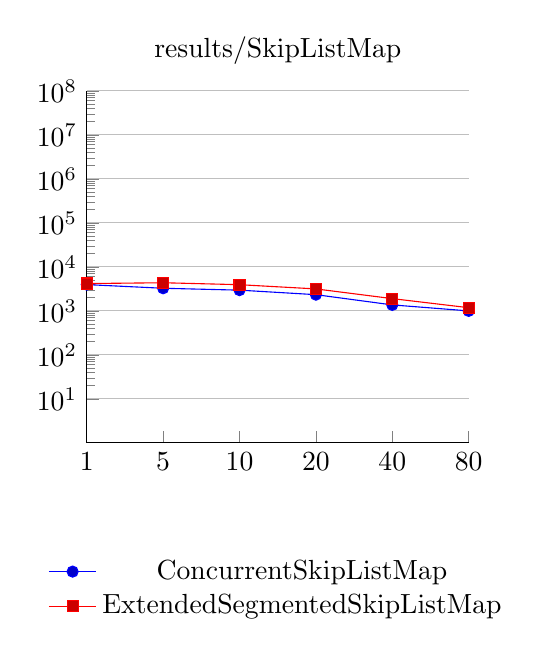
\begin{tikzpicture}[baseline={(current axis.north)}]
            \begin{axis}[
    xticklabels={1,5,10,20,40,80},
    xtick={1,2,3,4,5,6},
    ytick={0,10,1.0E2,1.0E3,1.0E4,1.0E5,1.0E6,1.0E7,1.0E8,1.0E9,1.0E10,1.0E11},
    ymin=1,
    ymax=100000000,
    xmin=1,
    xmax=6,
    y=0.02\textwidth,
    x=0.08\textwidth,
    ymode=log,
    log origin=0,
    ymajorgrids,
    axis x line*=bottom,
    axis y line*=left,
    ylabel style={font=\normalsize},
    xlabel style={font=\normalsize},
    title style={font=\normalsize},
    tick label style={font=\normalsize},
    legend style={draw=none, at={(0.5,-0.3)}, anchor=north,font=\normalsize},
    title=results/SkipListMap]
    \addplot coordinates {
       (1, 3949)
       (2, 3261)
       (3, 2954)
       (4, 2331)
       (5, 1364)
       (6, 997)
   };

    \addplot coordinates {
       (1, 4169)
       (2, 4354)
       (3, 3931)
       (4, 3151)
       (5, 1896)
       (6, 1179)
   };

  \legend{ConcurrentSkipListMap, ExtendedSegmentedSkipListMap, };
\end{axis}
            \end{tikzpicture}
            \\
            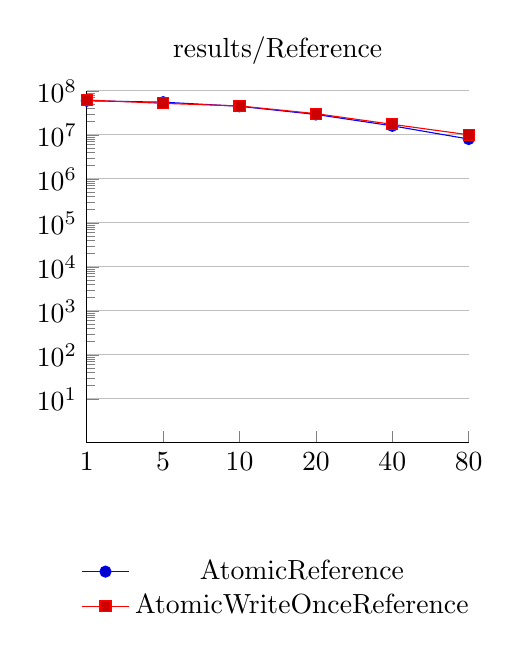
\begin{tikzpicture}[baseline={(current axis.north)}]
            \begin{axis}[
    xticklabels={1,5,10,20,40,80},
    xtick={1,2,3,4,5,6},
    ytick={0,10,1.0E2,1.0E3,1.0E4,1.0E5,1.0E6,1.0E7,1.0E8,1.0E9,1.0E10,1.0E11},
    ymin=1,
    ymax=100000000,
    xmin=1,
    xmax=6,
    y=0.02\textwidth,
    x=0.08\textwidth,
    ymode=log,
    log origin=0,
    ymajorgrids,
    axis x line*=bottom,
    axis y line*=left,
    ylabel style={font=\normalsize},
    xlabel style={font=\normalsize},
    title style={font=\normalsize},
    tick label style={font=\normalsize},
    legend style={draw=none, at={(0.5,-0.3)}, anchor=north,font=\normalsize},
    title=results/Reference]
    \addplot coordinates {
       (1, 59699629)
       (2, 55567915)
       (3, 44762626)
       (4, 29199671)
       (5, 16107761)
       (6, 8066552)
   };

    \addplot coordinates {
       (1, 62221648)
       (2, 52241644)
       (3, 45587119)
       (4, 30480623)
       (5, 17410687)
       (6, 10060201)
   };

  \legend{AtomicReference, AtomicWriteOnceReference, };
\end{axis}
            \end{tikzpicture}
            &
            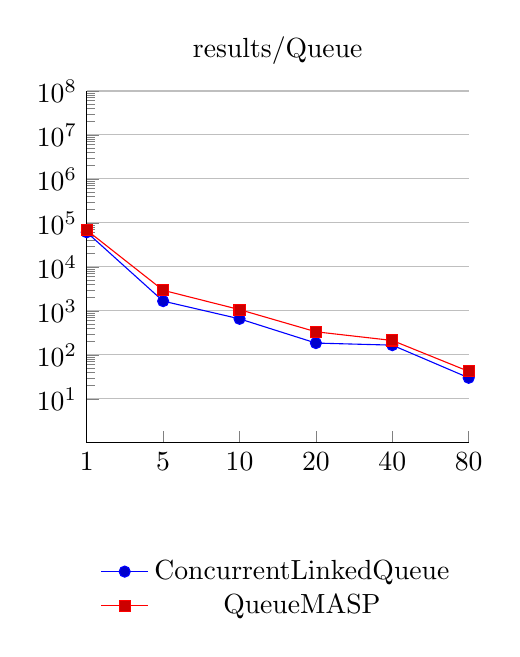
\begin{tikzpicture}[baseline={(current axis.north)}]
            \begin{axis}[
    xticklabels={1,5,10,20,40,80},
    xtick={1,2,3,4,5,6},
    ytick={0,10,1.0E2,1.0E3,1.0E4,1.0E5,1.0E6,1.0E7,1.0E8,1.0E9,1.0E10,1.0E11},
    ymin=1,
    ymax=100000000,
    xmin=1,
    xmax=6,
    y=0.02\textwidth,
    x=0.08\textwidth,
    ymode=log,
    log origin=0,
    ymajorgrids,
    axis x line*=bottom,
    axis y line*=left,
    ylabel style={font=\normalsize},
    xlabel style={font=\normalsize},
    title style={font=\normalsize},
    tick label style={font=\normalsize},
    legend style={draw=none, at={(0.5,-0.3)}, anchor=north,font=\normalsize},
    title=results/Queue]
    \addplot coordinates {
       (1, 61134)
       (2, 1663)
       (3, 658)
       (4, 185)
       (5, 166)
       (6, 30)
   };

    \addplot coordinates {
       (1, 68249)
       (2, 2932)
       (3, 1067)
       (4, 334)
       (5, 212)
       (6, 42)
   };

  \legend{ConcurrentLinkedQueue, QueueMASP, };
\end{axis}
            \end{tikzpicture}
            \\
        \end{tabular}
        ~~~~
        \caption{
            Performance of the objects in DEGO versus their counterparts in java.util.concurrent under high contention.
        }
    \end{figure}

    \begin{figure}
        \hspace{-8.8em}
        \begin{tabular}[t]{c c}
            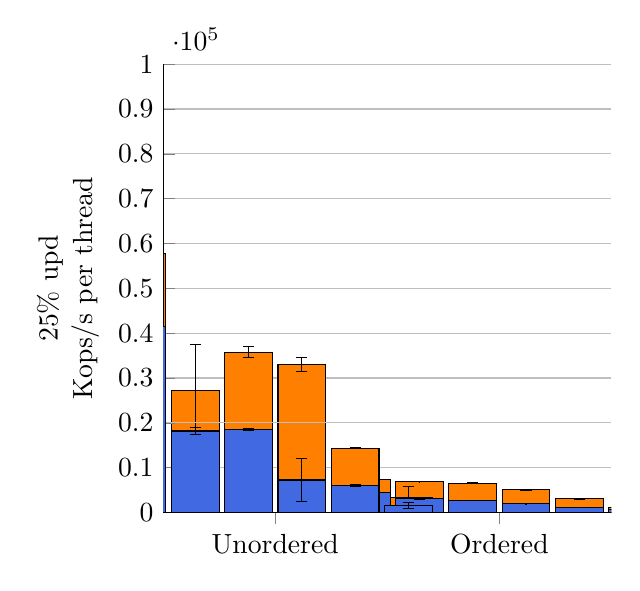
\begin{tikzpicture}
                \begin{axis}[
    ybar,
    width=0.6\linewidth,
    height=0.6\textwidth,
    bar width=0.05\linewidth,
    ylabel={\shortstack{25\% upd \\ Kops/s per thread}},
    ytick={0, 1.0E4, 2.0E4, 3.0E4, 4.0E4, 5.0E4, 6.0E4, 7.0E4, 8.0E4, 9.0E4, 1.0E5},
    ymin=0,
    ymax=100000,
    symbolic x coords={LeftMargin, Unordered, Space, Ordered, RightMargin},
    ymajorgrids,
    axis x line*=bottom,
    axis y line*=left,
    xtick=data,
    legend style={draw=none, at={(0.8,1.3)}, anchor=north, font=\normalsize},
    xmin=LeftMargin,
    xmax=RightMargin,
    ylabel style={font=\normalsize},
    xlabel style={font=\normalsize},
    title style={font=\normalsize},
    tick label style={font=\normalsize},
    cycle list={ {fill=orange}, {fill=orange} },
    area legend,
]
    \addplot+[error bars/.cd, y dir=both, y explicit] coordinates {
        (Unordered,57769) +- (683, 683) 
        (Ordered,7392) +-(364, 364)
    };

    \addplot+[error bars/.cd, y dir=both, y explicit] coordinates {
        (Unordered,27306) +- (10200, 10199) 
        (Ordered,6878) +-(48, 47)
    };

    \addplot+[error bars/.cd, y dir=both, y explicit] coordinates {
        (Unordered,35746) +- (1257, 1257) 
        (Ordered,6559) +-(97, 97)
    };

    \addplot+[error bars/.cd, y dir=both, y explicit] coordinates {
        (Unordered,32994) +- (1580, 1579) 
        (Ordered,5066) +-(38, 38)
    };

    \addplot+[error bars/.cd, y dir=both, y explicit] coordinates {
        (Unordered,14349) +- (93, 93) 
        (Ordered,3043) +-(44, 44)
    };

    \addplot+[error bars/.cd, y dir=both, y explicit] coordinates {
        (Unordered,3331) +- (2449, 2448) 
        (Ordered,1119) +-(104, 103)
    };

\end{axis}

\begin{axis}[
    ybar,
    width=0.6\linewidth,
    height=0.6\textwidth,
    bar width=0.05\linewidth,
    ymin=0,
    ymax=100000,
    symbolic x coords={LeftMargin, Unordered, Space, Ordered, RightMargin},
    ymajorgrids,
    axis x line*=bottom,
    axis y line*=left,
    xtick=data,
    legend style={draw=none, at={(0.9,1.2)}, anchor=north, font=\normalsize},
    xmin=LeftMargin,
    xmax=RightMargin,
    ylabel style={font=\normalsize},
    xlabel style={font=\normalsize},
    title style={font=\normalsize},
    tick label style={font=\normalsize},
    cycle list={ {fill=MyRoyalBlue}, {fill=MyRoyalBlue} },
    area legend,
    yticklabel={\empty},
    xticklabel={\empty},
    scaled y ticks=false,
]
    \addplot+[error bars/.cd, y dir=both, y explicit] coordinates {
        (Unordered,41592) +- (28, 28) 
        (Ordered,4456) +-(126, 125)
    };

    \addplot+[error bars/.cd, y dir=both, y explicit] coordinates {
        (Unordered,18186) +- (696, 695) 
        (Ordered,3120) +-(291, 291)
    };

    \addplot+[error bars/.cd, y dir=both, y explicit] coordinates {
        (Unordered,18532) +- (238, 237) 
        (Ordered,2702) +-(65, 64)
    };

    \addplot+[error bars/.cd, y dir=both, y explicit] coordinates {
        (Unordered,7249) +- (4804, 4803) 
        (Ordered,1928) +-(7, 7)
    };

    \addplot+[error bars/.cd, y dir=both, y explicit] coordinates {
        (Unordered,6122) +- (220, 221) 
        (Ordered,1153) +-(23, 23)
    };

    \addplot+[error bars/.cd, y dir=both, y explicit] coordinates {
        (Unordered,1535) +- (658, 658) 
        (Ordered,753) +-(26, 26)
    };

\end{axis}
            \end{tikzpicture}
            &
            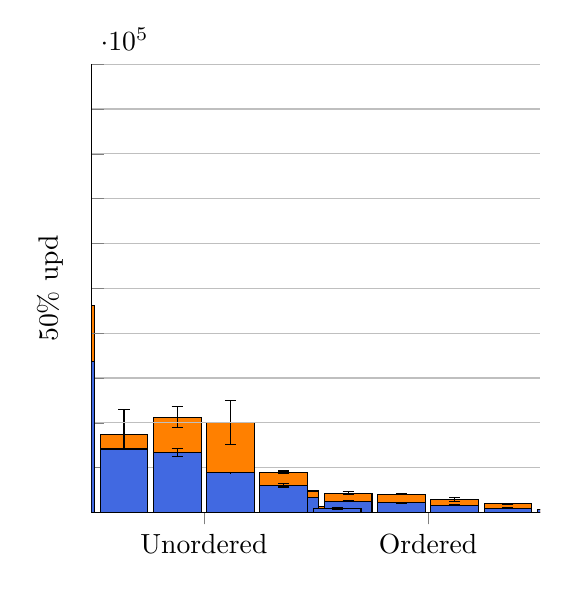
\begin{tikzpicture}
                \begin{axis}[
    ybar,
    width=0.6\linewidth,
    height=0.6\textwidth,
    bar width=0.05\linewidth,
    ylabel={50\% upd},
    yticklabel={\empty},
    ytick={0, 1.0E4, 2.0E4, 3.0E4, 4.0E4, 5.0E4, 6.0E4, 7.0E4, 8.0E4, 9.0E4, 1.0E5},
    ymin=0,
    ymax=100000,
    symbolic x coords={LeftMargin, Unordered, Space, Ordered, RightMargin},
    ymajorgrids,
    axis x line*=bottom,
    axis y line*=left,
    xtick=data,
    legend style={draw=none, at={(0.8,1.3)}, anchor=north, font=\normalsize},
    xmin=LeftMargin,
    xmax=RightMargin,
    ylabel style={font=\normalsize},
    xlabel style={font=\normalsize},
    title style={font=\normalsize},
    tick label style={font=\normalsize},
    cycle list={ {fill=orange}, {fill=orange} },
    area legend,
]
    \addplot+[error bars/.cd, y dir=both, y explicit] coordinates {
        (Unordered,46237) +- (1487, 1487) 
        (Ordered,4795) +-(50, 50)
    };

    \addplot+[error bars/.cd, y dir=both, y explicit] coordinates {
        (Unordered,17430) +- (5609, 5609) 
        (Ordered,4339) +-(261, 260)
    };

    \addplot+[error bars/.cd, y dir=both, y explicit] coordinates {
        (Unordered,21257) +- (2325, 2324) 
        (Ordered,4084) +-(142, 142)
    };

    \addplot+[error bars/.cd, y dir=both, y explicit] coordinates {
        (Unordered,20080) +- (4840, 4839) 
        (Ordered,2936) +-(452, 452)
    };

    \addplot+[error bars/.cd, y dir=both, y explicit] coordinates {
        (Unordered,9005) +- (256, 256) 
        (Ordered,1925) +-(57, 56)
    };

    \addplot+[error bars/.cd, y dir=both, y explicit] coordinates {
        (Unordered,1368) +- (53, 52) 
        (Ordered,687) +-(183, 183)
    };

\end{axis}

\begin{axis}[
    ybar,
    width=0.6\linewidth,
    height=0.6\textwidth,
    bar width=0.05\linewidth,
    ymin=0,
    ymax=100000,
    symbolic x coords={LeftMargin, Unordered, Space, Ordered, RightMargin},
    ymajorgrids,
    axis x line*=bottom,
    axis y line*=left,
    xtick=data,
    legend style={draw=none, at={(0.9,1.2)}, anchor=north, font=\normalsize},
    xmin=LeftMargin,
    xmax=RightMargin,
    ylabel style={font=\normalsize},
    xlabel style={font=\normalsize},
    title style={font=\normalsize},
    tick label style={font=\normalsize},
    cycle list={ {fill=MyRoyalBlue}, {fill=MyRoyalBlue} },
    area legend,
    yticklabel={\empty},
    xticklabel={\empty},
    scaled y ticks=false,
]
    \addplot+[error bars/.cd, y dir=both, y explicit] coordinates {
        (Unordered,33653) +- (38, 38) 
        (Ordered,3373) +-(167, 166)
    };

    \addplot+[error bars/.cd, y dir=both, y explicit] coordinates {
        (Unordered,14179) +- (15, 15) 
        (Ordered,2541) +-(117, 117)
    };

    \addplot+[error bars/.cd, y dir=both, y explicit] coordinates {
        (Unordered,13310) +- (873, 872) 
        (Ordered,2141) +-(44, 43)
    };

    \addplot+[error bars/.cd, y dir=both, y explicit] coordinates {
        (Unordered,8893) +- (17, 17) 
        (Ordered,1641) +-(83, 82)
    };

    \addplot+[error bars/.cd, y dir=both, y explicit] coordinates {
        (Unordered,6052) +- (354, 354) 
        (Ordered,992) +-(28, 27)
    };

    \addplot+[error bars/.cd, y dir=both, y explicit] coordinates {
        (Unordered,983) +- (209, 209) 
        (Ordered,650) +-(26, 25)
    };

\end{axis}
            \end{tikzpicture}
            \\
            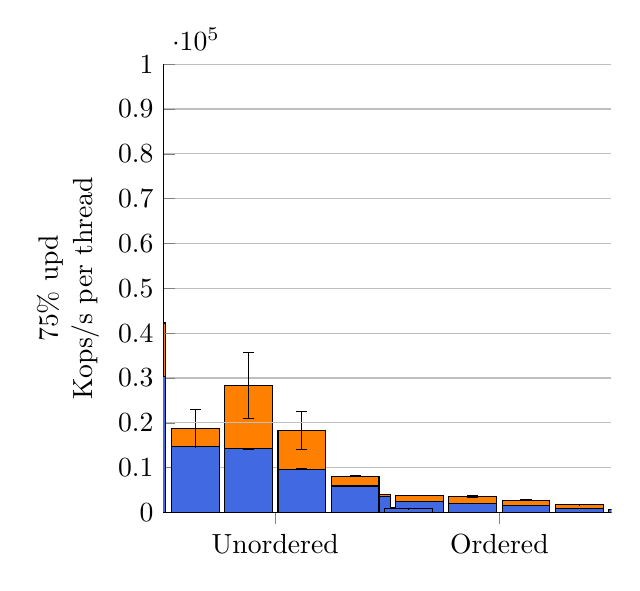
\begin{tikzpicture}
                \begin{axis}[
    ybar,
    width=0.6\linewidth,
    height=0.6\textwidth,
    bar width=0.05\linewidth,
    ylabel={\shortstack{75\% upd \\ Kops/s per thread}},
    ytick={0, 1.0E4, 2.0E4, 3.0E4, 4.0E4, 5.0E4, 6.0E4, 7.0E4, 8.0E4, 9.0E4, 1.0E5},
    ymin=0,
    ymax=100000,
    symbolic x coords={LeftMargin, Unordered, Space, Ordered, RightMargin},
    ymajorgrids,
    axis x line*=bottom,
    axis y line*=left,
    xtick=data,
    legend style={draw=none, at={(0.8,1.3)}, anchor=north, font=\normalsize},
    xmin=LeftMargin,
    xmax=RightMargin,
    ylabel style={font=\normalsize},
    xlabel style={font=\normalsize},
    title style={font=\normalsize},
    tick label style={font=\normalsize},
    cycle list={ {fill=orange}, {fill=orange} },
    area legend,
]
    \addplot+[error bars/.cd, y dir=both, y explicit] coordinates {
        (Unordered,42281) +- (2039, 2038) 
        (Ordered,4028) +-(34, 34)
    };

    \addplot+[error bars/.cd, y dir=both, y explicit] coordinates {
        (Unordered,18824) +- (4242, 4241) 
        (Ordered,3801) +-(1, 1)
    };

    \addplot+[error bars/.cd, y dir=both, y explicit] coordinates {
        (Unordered,28296) +- (7333, 7333) 
        (Ordered,3571) +-(106, 105)
    };

    \addplot+[error bars/.cd, y dir=both, y explicit] coordinates {
        (Unordered,18295) +- (4226, 4225) 
        (Ordered,2721) +-(73, 74)
    };

    \addplot+[error bars/.cd, y dir=both, y explicit] coordinates {
        (Unordered,8121) +- (164, 164) 
        (Ordered,1700) +-(6, 5)
    };

    \addplot+[error bars/.cd, y dir=both, y explicit] coordinates {
        (Unordered,1174) +- (110, 109) 
        (Ordered,748) +-(40, 39)
    };

\end{axis}

\begin{axis}[
    ybar,
    width=0.6\linewidth,
    height=0.6\textwidth,
    bar width=0.05\linewidth,
    ymin=0,
    ymax=100000,
    symbolic x coords={LeftMargin, Unordered, Space, Ordered, RightMargin},
    ymajorgrids,
    axis x line*=bottom,
    axis y line*=left,
    xtick=data,
    legend style={draw=none, at={(0.9,1.2)}, anchor=north, font=\normalsize},
    xmin=LeftMargin,
    xmax=RightMargin,
    ylabel style={font=\normalsize},
    xlabel style={font=\normalsize},
    title style={font=\normalsize},
    tick label style={font=\normalsize},
    cycle list={ {fill=MyRoyalBlue}, {fill=MyRoyalBlue} },
    area legend,
    yticklabel={\empty},
    xticklabel={\empty},
    scaled y ticks=false,
]
    \addplot+[error bars/.cd, y dir=both, y explicit] coordinates {
        (Unordered,30270) +- (108, 107) 
        (Ordered,3569) +-(244, 244)
    };

    \addplot+[error bars/.cd, y dir=both, y explicit] coordinates {
        (Unordered,14669) +- (21, 21) 
        (Ordered,2514) +-(6, 5)
    };

    \addplot+[error bars/.cd, y dir=both, y explicit] coordinates {
        (Unordered,14214) +- (46, 45) 
        (Ordered,2065) +-(34, 34)
    };

    \addplot+[error bars/.cd, y dir=both, y explicit] coordinates {
        (Unordered,9646) +- (108, 107) 
        (Ordered,1652) +-(8, 7)
    };

    \addplot+[error bars/.cd, y dir=both, y explicit] coordinates {
        (Unordered,5927) +- (196, 196) 
        (Ordered,953) +-(21, 21)
    };

    \addplot+[error bars/.cd, y dir=both, y explicit] coordinates {
        (Unordered,834) +- (26, 25) 
        (Ordered,657) +-(26, 25)
    };

\end{axis}
            \end{tikzpicture}
            &
            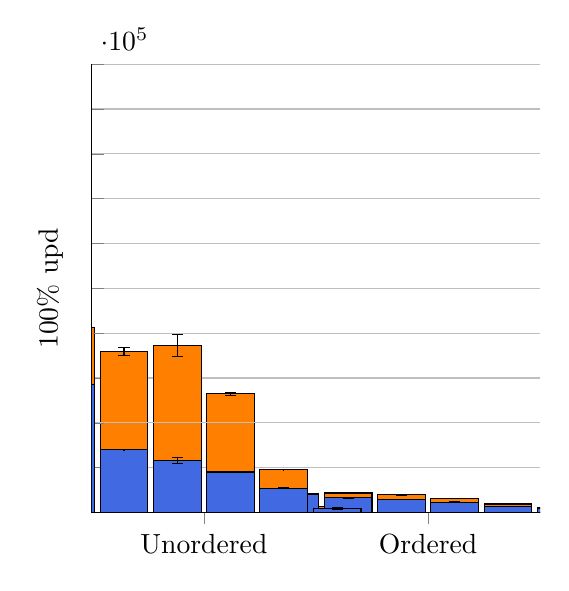
\begin{tikzpicture}
                \begin{axis}[
    ybar,
    width=0.6\linewidth,
    height=0.6\textwidth,
    bar width=0.05\linewidth,
    ylabel={100\% upd},
    yticklabel={\empty},
    ytick={0, 1.0E4, 2.0E4, 3.0E4, 4.0E4, 5.0E4, 6.0E4, 7.0E4, 8.0E4, 9.0E4, 1.0E5},
    ymin=0,
    ymax=100000,
    symbolic x coords={LeftMargin, Unordered, Space, Ordered, RightMargin},
    ymajorgrids,
    axis x line*=bottom,
    axis y line*=left,
    xtick=data,
    legend style={draw=none, at={(0.8,1.3)}, anchor=north, font=\normalsize},
    xmin=LeftMargin,
    xmax=RightMargin,
    ylabel style={font=\normalsize},
    xlabel style={font=\normalsize},
    title style={font=\normalsize},
    tick label style={font=\normalsize},
    cycle list={ {fill=orange}, {fill=orange} },
    area legend,
]
    \addplot+[error bars/.cd, y dir=both, y explicit] coordinates {
        (Unordered,41347) +- (19, 19) 
        (Ordered,4169) +-(307, 307)
    };

    \addplot+[error bars/.cd, y dir=both, y explicit] coordinates {
        (Unordered,35924) +- (928, 927) 
        (Ordered,4354) +-(9, 9)
    };

    \addplot+[error bars/.cd, y dir=both, y explicit] coordinates {
        (Unordered,37349) +- (2480, 2479) 
        (Ordered,3931) +-(140, 139)
    };

    \addplot+[error bars/.cd, y dir=both, y explicit] coordinates {
        (Unordered,26451) +- (389, 388) 
        (Ordered,3151) +-(28, 27)
    };

    \addplot+[error bars/.cd, y dir=both, y explicit] coordinates {
        (Unordered,9556) +- (23, 23) 
        (Ordered,1896) +-(142, 142)
    };

    \addplot+[error bars/.cd, y dir=both, y explicit] coordinates {
        (Unordered,1370) +- (26, 25) 
        (Ordered,1179) +-(20, 19)
    };

\end{axis}

\begin{axis}[
    ybar,
    width=0.6\linewidth,
    height=0.6\textwidth,
    bar width=0.05\linewidth,
    ymin=0,
    ymax=100000,
    symbolic x coords={LeftMargin, Unordered, Space, Ordered, RightMargin},
    ymajorgrids,
    axis x line*=bottom,
    axis y line*=left,
    xtick=data,
    legend style={draw=none, at={(0.9,1.2)}, anchor=north, font=\normalsize},
    xmin=LeftMargin,
    xmax=RightMargin,
    ylabel style={font=\normalsize},
    xlabel style={font=\normalsize},
    title style={font=\normalsize},
    tick label style={font=\normalsize},
    cycle list={ {fill=MyRoyalBlue}, {fill=MyRoyalBlue} },
    area legend,
    yticklabel={\empty},
    xticklabel={\empty},
    scaled y ticks=false,
]
    \addplot+[error bars/.cd, y dir=both, y explicit] coordinates {
        (Unordered,28632) +- (98, 98) 
        (Ordered,3949) +-(48, 47)
    };

    \addplot+[error bars/.cd, y dir=both, y explicit] coordinates {
        (Unordered,14003) +- (26, 26) 
        (Ordered,3261) +-(89, 88)
    };

    \addplot+[error bars/.cd, y dir=both, y explicit] coordinates {
        (Unordered,11587) +- (659, 658) 
        (Ordered,2954) +-(51, 50)
    };

    \addplot+[error bars/.cd, y dir=both, y explicit] coordinates {
        (Unordered,9030) +- (10, 9) 
        (Ordered,2331) +-(10, 9)
    };

    \addplot+[error bars/.cd, y dir=both, y explicit] coordinates {
        (Unordered,5444) +- (101, 101) 
        (Ordered,1364) +-(9, 9)
    };

    \addplot+[error bars/.cd, y dir=both, y explicit] coordinates {
        (Unordered,895) +- (254, 254) 
        (Ordered,997) +-(28, 28)
    };

\end{axis}
            \end{tikzpicture}
            \\
        \end{tabular}
        \caption{
            Varying the update ratio for a hash table (Unordered) and a skip list (Ordered).
        }
    \end{figure}

    \begin{figure}
        \begin{tikzpicture}
            \begin{axis}[
    width=\linewidth,
    height=0.5\textwidth,
    bar width=0.05\linewidth,
    ybar,
    ylabel={Kop/s per process},
    ytick={0, 1.0E4, 2.0E4, 3.0E4, 4.0E4, 5.0E4, 6.0E4, 7.0E4, 8.0E4, 9.0E4, 1.0E5},
    ymin=0,
    ymax=100000,
    ymajorgrids,
    axis x line*=bottom,
    axis y line*=left,
    xtick={0,1,2},
    xticklabels={16K,32K,64K},
    legend style={draw=none, at={(0.8,1.05)}, anchor=north, font=\normalsize},
    enlarge x limits=0.3,
    cycle list={ {fill=orange}, {fill=orange} },
    area legend,
    ylabel style={font=\normalsize},
    xlabel style={font=\normalsize},
    title style={font=\normalsize},
    y tick label style={font=\normalsize},
    x tick label style={font=\normalsize},
]
\addplot+[nodes near coords, point meta=explicit symbolic, every node near coord/.append style={yshift=6pt, xshift=-0.1cm, rotate=45, anchor=west, font=\normalsize}, error bars/.cd, y dir=both, y explicit] coordinates {
 (0,41347) +- (19, 19) 
 (1,41546) +- (30, 30) 
 (2,42131) +- (224, 223) 
};
\addplot+[nodes near coords, point meta=explicit symbolic, every node near coord/.append style={yshift=6pt, xshift=-0.1cm, rotate=45, anchor=west, font=\normalsize}, error bars/.cd, y dir=both, y explicit] coordinates {
 (0,35924) +- (928, 927) 
 (1,37545) +- (2041, 2040) 
 (2,35854) +- (490, 490) 
};
\addplot+[nodes near coords, point meta=explicit symbolic, every node near coord/.append style={yshift=6pt, xshift=-0.1cm, rotate=45, anchor=west, font=\normalsize}, error bars/.cd, y dir=both, y explicit] coordinates {
 (0,37349) +- (2480, 2479) 
 (1,35058) +- (454, 454) 
 (2,34631) +- (1204, 1203) 
};
\addplot+[nodes near coords, point meta=explicit symbolic, every node near coord/.append style={yshift=6pt, xshift=-0.1cm, rotate=45, anchor=west, font=\normalsize}, error bars/.cd, y dir=both, y explicit] coordinates {
 (0,26451) +- (389, 388) 
 (1,26513) +- (144, 143) 
 (2,20028) +- (1926, 1926) 
};
\addplot+[nodes near coords, point meta=explicit symbolic, every node near coord/.append style={yshift=6pt, xshift=-0.1cm, rotate=45, anchor=west, font=\normalsize}, error bars/.cd, y dir=both, y explicit] coordinates {
 (0,9556) +- (23, 23) 
 (1,7642) +- (20, 19) 
 (2,8952) +- (1324, 1324) 
};
\addplot+[nodes near coords, point meta=explicit symbolic, every node near coord/.append style={yshift=6pt, xshift=-0.1cm, rotate=45, anchor=west, font=\normalsize}, error bars/.cd, y dir=both, y explicit] coordinates {
 (0,1370) +- (26, 25) 
 (1,1164) +- (152, 152) 
 (2,1099) +- (275, 274) 
};
\legend{DEG}
\end{axis}

\begin{axis}[
    width=\linewidth,
    height=0.5\textwidth,
    bar width=0.05\linewidth,
    ybar,
    ytick={0, 1.0E4, 2.0E4, 3.0E4, 4.0E4, 5.0E4, 6.0E4, 7.0E4, 8.0E4, 9.0E4, 1.0E5},
    ymin=0,
    ymax=100000,
    ymajorgrids,
    axis lines=none,
    axis y line*=left,
    xtick={0,1,2},
    xticklabels={16K,32K,64K},
    legend style={draw=none, at={(0.8,0.88)}, anchor=north, font=\normalsize}},
    enlarge x limits=0.3,
    cycle list={ {fill=MyRoyalBlue}, {fill=MyRoyalBlue} },
    area legend,
    ylabel style={font=\normalsize},
    xlabel style={font=\normalsize},
    title style={font=\normalsize},
    tick label style={font=\normalsize},
    yticklabel={\empty},
    xticklabel={\empty},
    scaled y ticks=false,
]
\addplot+[nodes near coords, point meta=explicit symbolic, every node near coord/.append style={yshift=3pt, xshift=-0.35cm, rotate=45, anchor=west, font=\normalsize}, error bars/.cd, y dir=both, y explicit]coordinates {
 (0,28632) +- (98, 98) 
 (1,28126) +-(117, 117) 
 (2,28034) +-(30, 30) 
};
\addplot+[nodes near coords, point meta=explicit symbolic, every node near coord/.append style={yshift=3pt, xshift=-0.35cm, rotate=45, anchor=west, font=\normalsize}, error bars/.cd, y dir=both, y explicit]coordinates {
 (0,14003) +- (26, 26) 
 (1,16610) +-(89, 89) 
 (2,18988) +-(387, 387) 
};
\addplot+[nodes near coords, point meta=explicit symbolic, every node near coord/.append style={yshift=3pt, xshift=-0.35cm, rotate=45, anchor=west, font=\normalsize}, error bars/.cd, y dir=both, y explicit]coordinates {
 (0,11587) +- (659, 658) 
 (1,12716) +-(156, 156) 
 (2,15408) +-(119, 119) 
};
\addplot+[nodes near coords, point meta=explicit symbolic, every node near coord/.append style={yshift=3pt, xshift=-0.35cm, rotate=45, anchor=west, font=\normalsize}, error bars/.cd, y dir=both, y explicit]coordinates {
 (0,9030) +- (10, 9) 
 (1,10401) +-(128, 128) 
 (2,11293) +-(36, 36) 
};
\addplot+[nodes near coords, point meta=explicit symbolic, every node near coord/.append style={yshift=3pt, xshift=-0.35cm, rotate=45, anchor=west, font=\normalsize}, error bars/.cd, y dir=both, y explicit]coordinates {
 (0,5444) +- (101, 101) 
 (1,5619) +-(122, 123) 
 (2,5058) +-(1328, 1328) 
};
\addplot+[nodes near coords, point meta=explicit symbolic, every node near coord/.append style={yshift=3pt, xshift=-0.35cm, rotate=45, anchor=west, font=\normalsize}, error bars/.cd, y dir=both, y explicit]coordinates {
 (0,895) +- (254, 254) 
 (1,937) +-(9, 9) 
 (2,932) +-(10, 9) 
};
\legend{JUC}
\end{axis}
        \end{tikzpicture}
        \vspace{-1em}%
        \caption{Performance of a hash table with various working sets (75\% of updates)}
        \vspace{-1em}%
    \end{figure}

    \begin{figure}
        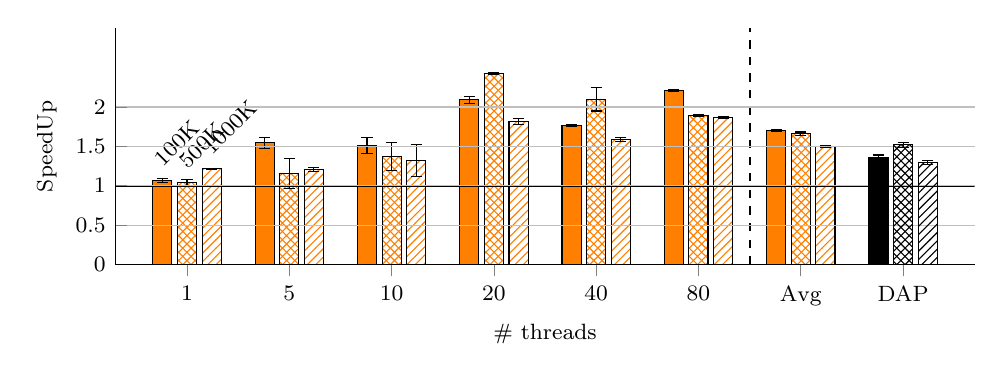
\begin{tikzpicture}
\begin{axis}[
    ybar,
    bar width=0.02\linewidth,
    ylabel={SpeedUp},
    ytick={0, 0.5, 1, 1.5, 2},
    ymin=0,
    ymax=3,
    xlabel={\# threads},
    xticklabels={1,5,10,20,40,80,Avg,DAP},
    xtick={0,1,2,3,4,5,6,7},
    scale only axis,
    width=0.9\linewidth,
    height = 3cm,
    ymajorgrids,
    axis x line*=bottom,
    axis y line*=left,
    legend style={draw=none, at={(0.5,1.2)}, anchor=north},
    cycle list=
        { 
        {pattern color=orange!100!white, fill=orange!100!white},
        {pattern color=orange!100!white, fill=orange!80!white, pattern=crosshatch},
        {pattern color=orange!100!white, fill=orange!60!white, pattern=north east lines},
        {pattern color=orange!100!white, fill=orange!40!white}
    }
        ,
    area legend,
    ylabel style={font=\footnotesize},
    xlabel style={font=\footnotesize},
    title style={font=\footnotesize},
    tick label style={font=\footnotesize}
]
        
\addplot+[nodes near coords, point meta=explicit symbolic, every node near coord/.append style={rotate=45, anchor=west, yshift=6pt, font=\footnotesize}, error bars/.cd, y dir=both, y explicit] coordinates {
 (0,1.066) +- (0.0234,0.0234) [100K]
 (1,1.5466) +- (0.0712,0.0712)
 (2,1.5115) +- (0.1005,0.1005)
 (3,2.0922) +- (0.0437,0.0437)
 (4,1.7684) +- (0.0117,0.0117)
 (5,2.2087) +- (0.0154,0.0154)
 (6,1.6989) +- (0.012,0.012)
 (7,0)
};

\addplot+[nodes near coords, point meta=explicit symbolic, every node near coord/.append style={rotate=45, anchor=west, yshift=6pt, font=\footnotesize}, error bars/.cd, y dir=both, y explicit] coordinates {
 (0,1.0375) +- (0.0394,0.0394) [500K]
 (1,1.1555) +- (0.1904,0.1904)
 (2,1.3705) +- (0.1825,0.1825)
 (3,2.4205) +- (0.0136,0.0136)
 (4,2.1002) +- (0.1509,0.1509)
 (5,1.8904) +- (0.0153,0.0153)
 (6,1.6624) +- (0.0203,0.0203)
 (7,0)
};

\addplot+[nodes near coords, point meta=explicit symbolic, every node near coord/.append style={rotate=45, anchor=west, yshift=6pt, font=\footnotesize}, error bars/.cd, y dir=both, y explicit] coordinates {
 (0,1.217) +- (0.0062,0.0062) [1000K]
 (1,1.2036) +- (0.0224,0.0224)
 (2,1.3164) +- (0.2039,0.2039)
 (3,1.8183) +- (0.0367,0.0367)
 (4,1.5852) +- (0.0286,0.0286)
 (5,1.8649) +- (0.0166,0.0166)
 (6,1.5009) +- (0.0151,0.0151)
 (7,0)
};
\draw[thick, black] (axis cs:-1,1) -- (axis cs:8,1);
\draw[dashed, thick, black] (axis cs:5.5,0) -- (axis cs:5.5,3);
\end{axis}

\begin{axis}[
    ybar,
    bar width=0.02\linewidth,
    ylabel={\empty},
    ytick={0, 0.5, 1, 1.5, 2},
    ymin=0,
    ymax=3,
    xlabel={\empty},
    xticklabels={1,5,10,20,40,80,Avg,DAP},
    xtick={0,1,2,3,4,5,6,7},
    scale only axis,
    width=0.9\linewidth,
    height = 3cm,
    ymajorgrids,
    axis x line*=bottom,
    axis y line*=left,
    legend style={draw=none, at={(0.5,1.2)}, anchor=north},
    cycle list=
        { 
        {pattern color=orange!100!white, fill=black!100!white},
        {pattern color=black!100!white, fill=black!80!white, pattern=crosshatch},
        {pattern color=black!100!white, fill=black!60!white, pattern=north east lines},
        {pattern color=black!100!white, fill=black!40!white}
    }
        ,
    area legend,
    ylabel style={font=\footnotesize},
    xlabel style={font=\footnotesize},
    title style={font=\footnotesize},
    tick label style={font=\footnotesize},
    yticklabel={\empty},
    xticklabel={\empty}
]
\addplot+[nodes near coords, point meta=explicit symbolic, every node near coord/.append style={rotate=45, anchor=west, yshift=6pt, font=\footnotesize}, error bars/.cd, y dir=both, y explicit] coordinates {
 (0,0)
 (1,0)
 (2,0)
 (3,0)
 (4,0)
 (5,0)
 (6,0)
 (7,1.36) +- (0.0304,0.0304)
};

\addplot+[nodes near coords, point meta=explicit symbolic, every node near coord/.append style={rotate=45, anchor=west, yshift=6pt, font=\footnotesize}, error bars/.cd, y dir=both, y explicit] coordinates {
 (0,0)
 (1,0)
 (2,0)
 (3,0)
 (4,0)
 (5,0)
 (6,0)
 (7,1.5191) +- (0.0283,0.0283)
};

\addplot+[nodes near coords, point meta=explicit symbolic, every node near coord/.append style={rotate=45, anchor=west, yshift=6pt, font=\footnotesize}, error bars/.cd, y dir=both, y explicit] coordinates {
 (0,0)
 (1,0)
 (2,0)
 (3,0)
 (4,0)
 (5,0)
 (6,0)
 (7,1.2925) +- (0.0238,0.0238)
};
\end{axis}
\end{tikzpicture}
        \caption{
            Performance of the social network application relative to the baseline (JUC).
        }
    \end{figure}

    \begin{figure}
        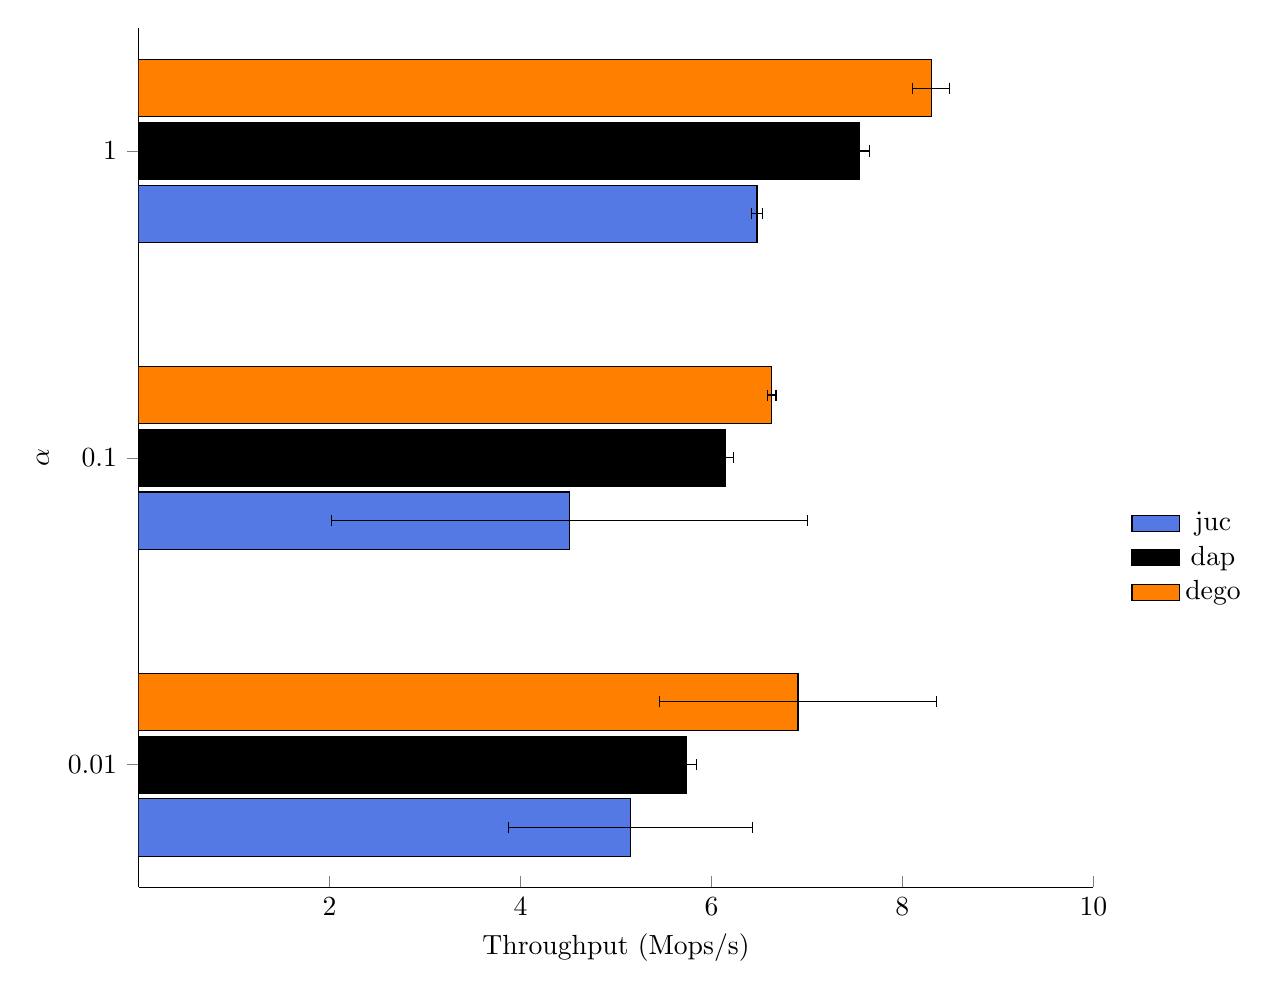
\begin{tikzpicture}
\begin{axis}[
        xbar,
        xlabel={Throughput (Mops/s)},
        xtick={2000, 4000, 6000, 8000, 10000},
        xticklabels={2, 4, 6, 8, 10},
        xmin=0,
        xmax=10000,
        height=0.9\textwidth,
        bar width=0.06\textwidth,
        width=\textwidth,
        ylabel={$\alpha$},
        yticklabels={0.01,0.1,1},
        ytick={0,1,2},
        scaled ticks=false,
        enlarge y limits=0.2,
        scale only axis,
        axis x line*=bottom,
        axis y line*=left,
        legend style={draw=none, at={(1.1,0.45)}, anchor=north},
        cycle list={ {fill=MyRoyalBlue!90!white},{fill=black}, {fill=orange} },
        area legend,]
        
\addplot+[error bars/.cd, x dir=both, x explicit] coordinates {
 (5149.5,0) +- (1276.94,1276.94)
 (4512.0,1) +- (2493.12,2493.12)
 (6477.5,2) +- (55.86,55.86)
};

\addplot+[error bars/.cd, x dir=both, x explicit] coordinates {
 (5737.0,0) +- (105.83999999999999,105.83999999999999)
 (6148.5,1) +- (79.38,79.38)
 (7549.5,2) +- (102.89999999999999,102.89999999999999)
};

\addplot+[error bars/.cd, x dir=both, x explicit] coordinates {
 (6906.0,0) +- (1448.44,1448.44)
 (6631.5,1) +- (44.099999999999994,44.099999999999994)
 (8300.0,2) +- (197.95999999999998,197.95999999999998)
};
\legend{juc,dap,dego}
\end{axis}
\end{tikzpicture}
        \caption{
            Varying the user access distribution.
        }
    \end{figure}
\end{document}